%%%%%%%%%%%%%%%%%%%%%%%%%%%%%%%%%%%%%%%%%%%%%%%%%%%%%%%%%%%%%%%%%%%%%%%%%%%%%%
%UNIVERSITA' DEGLI STUDI DI MILANO                                           %
%DIPARTIMENTO DI INFORMATICA                                                 %
%TESI DI LAUREA TRIENNALE IN SICUREZZA DEI SISTEMI E DELLE RETI INFORMATICHE %
%FRANCESCO AVANTAGGIATO MATR: 942790                                         %    
%%%%%%%%%%%%%%%%%%%%%%%%%%%%%%%%%%%%%%%%%%%%%%%%%%%%%%%%%%%%%%%%%%%%%%%%%%%%%%
\documentclass[12pt,italian]{report}
\usepackage{tesi}


% CORSO DI LAUREA:
\def\myCDL{Corso di Laurea in\\Sicurezza dei Sistemi e delle Reti Informatiche\\(L-31 Scienze e Tecnologie Informatiche) }

% TITOLO TESI:
\def\myTitle{Studio e sviluppo di connettori di scraping di sorgenti\\ social network per ingestione in sistemi di Big Data Analytics}

% AUTORE:
\def\myName{Francesco Avantaggiato}
\def\myMat{Matr. 942790}

% RELATORE 
\def\myRefereeA{Prof. Marco Anisetti}

% ANNO ACCADEMICO
\def\myYY{2021/2022}

\usepackage{afterpage}

\newcommand\blankpage{%
    \null
    \thispagestyle{empty}%
    \addtocounter{page}{-1}%
    \newpage}
% Package di formato
%\usepackage[a4paper]{geometry}		% Formato del foglio
\usepackage[italian]{babel}			% Supporto per l'italiano
\usepackage[utf8]{inputenc}			% Supporto per UTF-8
\usepackage[a-1b]{pdfx}			    % PDF-A (obbligatorio per la consegna)

% Package per la grafica
\usepackage{graphicx}				
\usepackage{hologo}					
\usepackage{svg}
\usepackage{listingsutf8}
\usepackage{minted}
\definecolor{bg}{rgb}{0.95,0.95,0.95}
\lstdefinelanguage{docker}{
  keywords={FROM, RUN, COPY, ADD, ENTRYPOINT, CMD,  ENV, ARG, WORKDIR, EXPOSE, LABEL, USER, VOLUME, STOPSIGNAL, ONBUILD, MAINTAINER},
  keywordstyle=\color{blue}\bfseries,
  identifierstyle=\color{black},
  sensitive=false,
  comment=[l]{\#},
  commentstyle=\color{purple}\ttfamily,
  stringstyle=\color{red}\ttfamily,
  morestring=[b]',
  morestring=[b]"
}
%\usepackage{epsfig}				
%\usepackage{xcolor}				

% Package tipografici
\usepackage{amssymb,amsmath,amsthm} 
\usepackage{listings}				
\usepackage{caption} 
\captionsetup[table]{skip=10pt}

% Package ipertesto
\usepackage{url}				
\usepackage{hyperref}				
\usepackage{pgfplots}
\pgfplotsset{width=10cm,compat=1.9}
\begin{document}



% Creazione automatica del frontespizio
\frontespizio
\beforepreface


{\raggedleft \large \sl 
	\vspace{6cm}

	
%dedica
	A mio Fratello
	\bigskip
	
	}


%Creazione automatica dell'indice
\afterpreface
%Capitolo 1: Introduzione
\chapter{Introduzione}

\label{cap:introduzione}
\section{Il progetto}
Il progetto sviluppato per questo lavoro di tesi ha riguardato l'attivit\`a del web scraping da fonti social network e la sua applicazione nella programmazione di connettori di dati in sistemi di Big Data Analytics. Lo studio di soluzioni valide ha individuato come obiettivi principali i social di Meta Inc., ovvero Facebook ed Instagram, per la loro vasta utenza e conseguente ingente quantit\`a di dati pubblici. 

Nella tesi vengono affrontate tematiche inerenti alla legalit\`a delle azioni di scraping, in quanto ad oggi, l'attivit\`a ricade in  una ``zona grigia'', non essendo previste direttamente norme. I social tramite i loro termini di servizio, vietano qualsiasi tipologia di estrazione dati, anche adottando soluzioni tecniche, per salvaguardare le informazioni pubblicate dai propri utenti.

Oggetto di attenzione all'interno del progetto \`e anche l'impiego dei dati estratti, presentando valide proposte d'utilizzo per scopi di investigazione e Open Source Intelligence.

Lo sforzo tecnico e progettuale \`e consistito principalmente nella creazione di valide metodologie di elusione dei controlli anti-scraping attuati dalle piattaforme. Lo studio del contrasto ha garantito la progettazione di sistemi attuabili in entrambi i connettori dei social target, uniformando la loro gestione e il loro output.


\section{Organizzazione dei contenuti}
Il presente lavoro di tesi \`e cos\`i strutturato: \\
Il Capitolo \ref{chap:stato_arte} presenta lo stato dell'arte rispetto al web scraping in generale e da fonti social network. Vengono inoltre citati gli scenari d'impiego dei dati in ambito investigativo e gli aspetti giuridici dell'attivit\`a. \\
Il Capitolo \ref{chap:analisi_concettuale} individua i requisiti di un progetto di web scraping presentando le tecnologie di base da impiegare, le soluzioni ideali di elusione dei controlli anti-scraping e la gestione dei dati in output.\\
Nel Capitolo \ref{chap:caso_studio} viene presentato il lavoro di studio e sviluppo svolto per il progetto di tesi. In particolare per i singoli connettori di Facebook ed Instagram vengono proposti i punti salienti del progetto e le soluzioni implementative attuate. Inoltre vengono elencate ed esplicate tutte le tecnologie di sviluppo adottate.\\
Il Capitolo \ref{chap:test} presenta i test effettuati sul software, proponendo un confronto sia sulle versioni dei tool open source impiegati che sull'efficienza in termini di dati, tempo e resistenza dei connettori sviluppati.\\
Nel Capitolo \ref{chap:conclusioni} vengono esposte le conclusioni sul progetto sviluppato, presentando eventuali sviluppi futuri. \\
Infine, nell'Appendice, \ref{appendice} sono presentate parti del codice prodotto ed esempi di output dei connettori. \\


\afterpage{\blankpage}

%Capitolo 2: Stato dell'arte
\chapter{Stato dell'arte}
\label{chap:stato_arte}
Le applicazioni di estrazione dati nel web aumentano esponenzialmente con il valore delle informazioni. La vasta eterogeneit\`a consente lo sviluppo e lo svolgimento di quest`attivit\`a in ambiti differenti. 

Ad oggi, porre come obiettivo di scraping un social network vuol dire catalogare e gestire enormi quantit\`a di dati. La presenza di interesse delle societ\`a e delle community open source al tema dello scraping dei social, individua l'importanza delle informazioni memorizzate su questi servizi e la conseguente protezione degli stessi da parte dei gestori delle piattaforme. 

Con la presenza di regolamentazioni e leggi a carattere statale ed internazionale si nota come i gestori dei servizi siano stati nel tempo obbligati a cambiare l'approccio nei confronti della gestione dei dati pubblici. Inoltre, la dichiarazione di particolari termini d'uso delle piattaforme, garantisce un'apparente protezione dell'utente nei confronti dell'utilizzo dei dati per scopi non previsti.

Nel seguente capitolo si presenter\`a lo stato dell'arte del web scraping, con particolare attenzione ai social network.
\newpage
\section{Web Scraping}
Con il termine ``web scraping'' si fa riferimento all'attivit\`a di raccolta automatica di informazioni da Internet inglobando sia varie tecniche di programmazione che diverse tecnologie web.
Solitamente l'acquisizione di dati da un servizio avviene attraverso le Application Programming Interface (paragrafo \ref{API}) messe a disposizione dallo stesso, in grado di fornire output formattati e standardizzati (es. JSON), pronti ad essere analizzati.\cite{mitchell2018web}

Nel campo della ricerca ed estrazione dei dati su internet, \`e necessario prendere in considerazione anche l'esistenza dell'attivit\`a nota come ``web crawling''. Il web crawling, a differenza dello scraping, viene impiegato per l'analisi e l'indicizzazione dei siti web ed utilizzato da parte dei motori di ricerca per fornire i risultati basati sulle parole chiave richieste dagli utenti. L'applicazione in grado di effettuare l'attivit\`a di crawling \`e definita ``web crawler'', nota anche come ``spider'' o ``robot''.\cite{olston2010web}

L'ingente quantit\`a di dati eterogenei presenti in Internet implica un maggiore interesse nello sviluppo di sistemi automatizzati di raccolta di informazioni. La possibilit\`a di estrapolazione ed analisi dati forniscono degli strumenti di lavoro applicabili in molti settori della societ\`a moderna. Si pensi ad esempio alla possibilit\`a di impiego dei dati per analisi statistiche, per marketing, per pubblicit\`a e per ricerche in genere.

La fruizione di dati relativi a singole persone, societ\`a, attivit\`a commerciali, contribuiscono alla alimentazione di sistemi di Big Data Analytics. Questi ultimi sono in grado di proporre strumenti di predizione ed analisi in chiave investigativa e di accelerare l'attivit\`a di Intelligence (nel particolare Virtual Intelligence).

Lo sviluppo di sistemi con un'operativit\`a temporale continua, crea conseguentemente un'attenta risposta di contrasto.
Ci\`o accade in quanto molto spesso l'impiego dell'attivit\`a di scraping avviene con fini malevoli e quindi considerata come ``furto di dati''. 
In particolare queste operazioni vengono esplicitamente proibite dai ToS \footnote{Terms of service} (termini di servizio) delle piattaforme web, soprattutto per ragioni di sicurezza delle informazioni e protezione dei dati pubblicati.

L'impiego di bot e botnet in grado di simulare e mascherare le operazioni automatizzate facendole apparire ``umane'', rappresenta la principale metodologia per lo scraping su larga scala. Precisamente l'avvio di un sistema distribuito avente pi\`u macchine con lo stesso obiettivo, permette di eludere agevolmente tutti gli eventuali controlli messi in atto dal fornitore dei servizi web per la protezione dei dati pubblicati. 

La variet\`a di soluzioni di scraping attuabili presenta punti di forza per la gestione di operazioni massive. Diversificando metodologie di estrazione, i bot possono agire contemporaneamente e svolgere attivit\`a specifiche e diversificate, a seconda del target individuato.

Un esempio di raccolta dati automatica viene rappresentato dalla generazione e messa in campo di sistemi e strumenti di automazione dei browser. Questi sono in grado, anche visivamente, di simulare la normale attivit\`a di un utente sul web, premendo pulsanti, caricando siti internet e procedendo all'inserimento di input, oltre che ovviamente, al download delle informazioni di interesse. 
%aggiungere altro ...


\begin{figure}[!htb]
  \begin{center}
  \includesvg[width=400pt]{immagini/scraper.svg}
  \caption{Schema di Web Scraping}
\end{center}
\end{figure}
%grafico generale funzionamento scraping dal web


\subsection{L'estrazione dei dati dai Social Network} \label{dati_social}
L'attivit\`a di scraping trova come importante campo d'applicazione i social network. Ad oggi, il vasto utilizzo di questi servizi porta alla registrazione di una moltitudine di dati diversi, caratterizzati dall'associazione degli stessi ad i singoli utenti. L'analisi della rete sociale di una persona, consente l'aggregazione dei dati e la sua conseguente profilazione.
L'etereogeneit\`a dei dati rappresenta il punto iniziale per la catalogazione delle informazioni provenienti dalle piattaforme social. Il valore dei social network \`e direttamente proporzionale alla quantit\`a di dati presenti.

L'attivit\`a denominata come ``social engagement'' ovvero il coinvolgimento degli utenti, fornisce un valido fattore di analisi sul comportamento che la singola persona attua di fronte ad un certo tipo di contenuto. Lo studio di queste informazioni garantisce una attenta profilazione dell'utente, molte volte inconsapevole della quantit\`a di dati pubblici rilasciati dalla sua attivit\`a sui social.

Ogni piattaforma social a disposizione del pubblico adotta policy differenti riguardo alla estrazione dei dati. In particolare se da un lato vengono fornite Application Programming Interface appositamente sviluppate per la fruizione pi\`u semplice delle informazioni da parte degli sviluppatori, dall'altro si ha l'adozione di politiche restrittive, con API molto limitate ed un netto contrasto ai tentativi di estrapolazione dei dati. 
Negli ultimi anni, a seguito di clamorose notizie riguardanti l'utilizzo dei dati a discapito della privacy degli utenti, \`e diventato comune da parte delle piattaforme social l'introduzione di forti restrizioni sull'attivit\`a di scraping, attuando un vero e proprio contrasto a questo tipo di attivit\`a.

La presenza di un numero cos\`i grande di PII\footnote{Personally identifiable information}, ovvero qualsiasi rappresentazione di informazioni in grado di consentire l'identificazione di un individuo, ha generato maggiore attenzione sulla privatezza delle informazioni pubblicate dagli utenti, a tutela dei loro dati.\cite{isaak2018user}

L'identificazione di metriche idonee per lo sviluppo e l'analisi dei dati pubblicati si pu\`o classificare a seconda degli obiettivi di ricerca: 
\begin{itemize}
    \item \textbf{Volume dei dati}: un profilo con una grande influenza sul web pu\`o contenere fino a migliaia di contenuti di interesse operativo.
    \item \textbf{Testi}: i testi contenuti all'interno di post o all'interno di foto e video possono descrivere pensieri e sentimenti dell'utente.
    \item \textbf{Media}: le foto e i video pubblicati rappresentano un elemento fondamentale per l'analisi e la profilazione. L'eventuale presenza di luoghi o altre persone nei media garantisce una maggiore quantit\`a di informazioni da immagazzinare ed analizzare.
    \item \textbf{Individui coinvolti}: l'azione del ``tag'' su una foto, video o su un post composto da solo testo, consente di ampliare la conoscenza su un utente, azionando il recupero delle informazioni anche su eventuali altri individui coinvolti.
    \item \textbf{Reazioni e commenti}: contribuiscono ad interpretare la diffusione di un messaggio o ideale propagato sul social network. Un alto numero \`e direttamente proporzionale all'interesse generato dal contenuto.
    \item \textbf{Geolocalizzazione}: la condivisione della posizione, correlata dalla specifica data ed ora, consente di identificare gli spostamenti o gli interessi di un utente, aumentando la precisione della sua eventuale profilazione.
    \item \textbf{Date e tempo}: l'estrazione di informazioni in un certo arco temporale d'interesse o la redazione di una totale cronostoria del profilo social favorisce l'individuazione di informazioni relative ad uno specifico periodo.
    \item \textbf{Rete sociale}: l'insieme degli amici o dei follower e dei seguiti, rappresenta la rete sociale dell'utente e gli eventuali interessi.
    \item \textbf{Gruppi di utenti}: la partecipazione a gruppi privati o pubblici presenta informazioni aggiuntive sull'individuo.
    \item \textbf{Pagine}: interesse verso pagine pubbliche di diversa tipologia (ad esempio notizie o brand).
    \item \textbf{Eventi}: partecipazione a manifestazioni, interesse nei confronti di eventi pubblici.
    
\end{itemize}
L'interpretazione di questi fattori, sia singolarmente che in gruppo individuano le informazioni di interesse per chi analizza i dati. Un numero maggiore di aggregazioni e correlazioni dei dati, genera una profilazione dell'utente pi\`u precisa ed utile.
\begin{figure}[!htb]
  \begin{center}
  \includesvg[width=400pt]{immagini/schema_social.svg}
  \caption{Schema di funzionamento di un sistema ideale di ricerca analisi ed estrazione dei dati da social network}
\end{center}
\end{figure}


\subsection{Casi reali} \label{casi_reali}
Un esempio di notizia nota al pubblico per la forte influenza mediatica \`e il caso di Cambridge Analytica e Facebook. All'inizio dell'anno 2018 fu rivelato che la societ\`a Cambridge Analytica aveva effettuato una massiva raccolta di dati (circa 87 milioni di account del social Facebook) con conseguente profilazione degli utenti ed impiegato i risultati per attivit\`a di propaganda politica.
La profilazione degli utenti avveniva attraverso l'utilizzo, da parte degli stessi, di un'app di ``quiz sulla personalit\`a'', tramite la quale ciascun fruitore dava il consenso all'accesso ai dati del profilo.

La profilazione avveniva secondo un modello denominato OCEAN\footnote{Anche denominata Teoria dei Big Five, \`e una tassonomia dei tratti di personalit\`a}: Openness (franchezza, apertura sociale), Conscientiousness (coscienziosit\`a), Extraversion (estroversione), Agreeableness (gradevolezza, amicalit\`a), Neuroticism (nevroticismo). 
Dal caso ne \`e derivata la chiusura dell'azienda per bancarotta, senza risvolti legali.\cite{tirino2019cambridge}

Un altro caso di impiego attivo di web scraping \`e il software sviluppato dall'azienda americana Clearview AI. Il prodotto consente l'identificazione delle persona tramite l'intelligenza artificiale, sfruttando database composti anche da informazioni e foto estratte dai social network. Negli anni, i maggiori social hanno richiesto l'eliminazione dei dati estratti dalla societ\`a, anche se quest'ultima ha sempre dichiarato che l'impiego del progetto sia dedicato alle forze dell'ordine. 

In Italia il Garante per la protezione dei dati personali, ha emesso in data 9 febbraio 2022 un'ordinanza di ingiunzione contro l'utilizzo di dati estratti da fonti pubbliche inerenti a cittadini italiani, sanzionando la societ\`a e vietandone la sua attivit\`a nello Stato Italiano. \footnote{\url{https://www.garanteprivacy.it/web/guest/home/docweb/-/docweb-display/docweb/9751362}}

Altre implicazione legali sono state causate dal caso di Linkedin ed hiQ Labs. Nel particolare quest'ultima attuava soluzioni di web scraping sulla piattaforma Linkedin, raccogliendo informazioni sui profili registrati al servizio. La corte d'appello degli Stati Uniti ha dato ragione all'azienda hiQ Labs ritenendo che l'estrazione di dati pubblici non sia illegale. Di contro, Linkedin contrastava la decisione affermando la necessit\`a di autorizzazioni per l'attivit\`a di scraping sulla loro piattaforma.
%aggiungere casi?

Le problematiche evidenziate dai casi descritti, hanno fatto s\`i che da parte delle piattaforme social, ci sia stato un conseguente forte incremento di soluzioni di sicurezza e contrasto al recupero ed estrazione dei dati non autorizzata.



\subsection{Metodologie di contrasto allo scraping} \label{metodi_contrasto}
Attualmente, anche se con modalit\`a differenti, ogni social adotta politiche di contrasto, ponendo come fulcro dell'attivit\`a la protezione dei dati personali dei propri utenti.
La mitigazione del web scraping adottata dai social network individua delle tecniche con caratteristiche comuni:
\begin{itemize}
    \item \textbf{Autenticazione ed accesso}: uno dei principali strumenti di deterrenza nei confronti dell'automazione dell'estrazione dei dati \`e l'obbligatoriet\`a di iscrizione al sito web ed il conseguente login.
    \item \textbf{Ban}: attuazione di politiche di divieto d'accesso per dispositivi ed utenze identificate come ``malevoli'' e non rispettanti i termini di servizio. Il possibile ban si distingue in ``soft-ban'' e ``permanent-ban'', a seconda delle policy di contrasto del servizio. Per soft-ban si fa riferimento ad un divieto di durata limitata nel tempo, solitamente definibile in ore o giorni, mentre per permanent-ban si intende un divieto assoluto e permanente all'accesso da parte di un determinato utente.
    \item \textbf{Robots Exclusion Standard}: rappresenta un protocollo di comunicazione tra i siti internet ed i web crawler. Il metodo esclude i robot dall'accesso al sito attraverso l'espressione di politiche d'acesso (access policy) all'interno di un file denominato ``robots.txt'' ed accessibile sul server. Il file \`e caratterizzato da pi\`u record composti dalla descrizione dello ``User Agent'' e dalla regola ``Disallow'' (lett. ``non consentire'')\footnote{\url{https://www.robotstxt.org/orig.html}}.
    
    Si riporta un esempio estratto dal file robots di Facebook\footnote{\url{https://www.facebook.com/robots.txt}}:
    \inputminted[bgcolor=bg]{text}{codice/robots.txt}
    \item \textbf{Limitazione delle API}: le API messe a disposizione per gli  sviluppatori presentano limitazioni sulla quantit\`a dei dati estraibili, non consentendo uno scraping completo o massivo.
    \item \textbf{Limitazione delle richieste}: le richieste provenienti da uno stesso dispositivo ed in un ristretto periodo temporale vengono attenzionate ed impedite. L'analisi automatica del numero di richieste consente di gestire in modo meccanico i processi di ban.
    \item \textbf{Controllo indirizzi IP}: controllo sulla provenienza della richiesta. Viene effettuato un controllo sulle richieste provenienti dallo stesso indirizzo IP (o pool di indirizzi IP), iscrivendolo eventualmente in blacklist e bloccando la sua attivit\`a. Ci\`o pu\`o avvenire sia relativamente ai singoli IP, sia alla provenienza da regioni geografiche simili o vicine.
    \item \textbf{Browser fingerprinting}: analisi remota delle informazioni di un dispositivo. Le informazioni del client ricavabili con questa tecnica indicano il browser utilizzato (con versione e personalizzazioni), sistema operativo e applicazioni, hardware e network.\cite{nikiforakis2013cookieless}
    \item \textbf{Identificatori pseudoanonimi}: l'attivit\`a di scraping si avvale dell'estrazione diretta dei dati a partire da un link, molte volte statico. Per evitare ci\`o viene prevista la presenza di ID pseudoanonimi\footnote{Si identificano come informazioni non completamente anonime} random generati a partire dall'ID fisso ed il timestamp\footnote{Anche denominata marca temporale, \`e una sequenza di caratteri che rappresentano una data e un orario ed in grado di accertare l'avvenimento di un evento}. Questo previene l'attivit\`a dei tool che sfruttano la staticit\`a dei link per avviare le operazioni di GET. 
    \item \textbf{Identificazione ``umana''}: alcuni social network per evitare che venga effettuato un login automatico da parte di bot, obbligano  all'identificazione di una persona reale, attraverso una foto da scattare sul momento.
    \item \textbf{Aggiornamenti}: continuo sviluppo di metodi di contrasto allo scraping. Creazione di team di sviluppo appositamente dedicati a questa funzione.
\end{itemize}
L'elenco delle attivit\`a sopra descritte rappresenta una sola parte dei provvedimenti che ad oggi vengono adottati per contrastare l'automazione nella raccolta dei dati. \`E importante rendere noto che per la maggior parte dei servizi web, la risposta allo scraping non implica solo una delle soluzioni descritte bens\`i l'insieme di almeno due o pi\`u ``ostacoli'' di tipo tecnico.
\section{L'utilizzo dei dati}
\subsection{Open Source Intelligence} \label{OSINT}
L'OSINT \cite{intelligence_guida} (Open source intelligence) rappresenta il ramo dell'intelligence che si occupa della ricerca e catalogazione delle informazioni da fonti aperte. Per fonti aperte si intendono i media, i dati pubblici ed i dati accademici. Questo tipo di attivit\`a sviluppa come vantaggio l'accessibilit\`a delle informazioni, le quali essendo pubbliche, risultano facilmente reperibili; mentre la quantit\`a di dati da gestire rappresenta il principale problema di questa tecnica.
L'applicazione dell'attivit\`a di intelligence su piattaforme social network prende il nome di ``Social media intelligence''.
\cite{gnosis_int}.

L'etereogeneit\`a dei dati pubblicati da un utente sulle piattaforme social, consente all'analista d'intelligence lo sviluppo di schemi di analisi comportamentali e sociali. La presenza di dati temporanei (``a scadenza''), come ad esempio le storie, fornisce informazioni in tempo reale sull'attivit\`a di un soggetto sottoposto a controllo.
Il tracciamento e la profilazione di un individuo si completa grazie ad informazioni che esso stessa pubblica come la geolocalizzazione, la sua rete sociale, i post e i media, le reazioni ed i commenti, oltre che agli interessi personali espressi tramite i ``mi piace'' e la sua attivit\`a nel complesso.
\`E importante fare presente che la principale fonte dell'OSINT non \`e rappresentata dal Worldwide Web ma dal Deep Web, ovvero la porzione di web non indicizzata dai motori di ricerca.
\subsection{Scenari d'impiego}
I dati raw, ``grezzi'', estratti dalle fonti pubbliche, una volta sottoposti ad ingestione in sistemi di Big Data Analytics e processati, possono essere analizzati tramite tecniche di Sentiment Analysis\footnote{Elaborazione del linguaggio naturale per l'estrazione di opinioni e sentimenti.}.
I dati prodotti, descritti al Paragrafo \ref{dati_social}, possono essere impiegati in molteplici attivit\`a come:
\begin{itemize}
    \item \textbf{Contrasto a radicalizzazione e terrorismo online}: le policy dei social network vietano la pubblicazione di contenuti relativi ad organizzazione terroristiche o a relative radicalizzazioni e di contenuti violenti, attuando, anche tramite lo strumento della segnalazione, l'eliminazione di questi dati. Ci\`o non avviene sempre in maniera immediata o corretta e per questo motivo, garantire un'estrazione dati continua e performante consentirebbe di ricavare informazioni che in futuro saranno sottoposte a controllo ed eliminazione.
    L'impiego da parte di gruppi sovversivi di piattaforme web di interazione sociale, facilita anche il processo di reclutamento, promuovendo ideali ed azioni in contrasto con la societ\`a moderna.
    Ci\`o consente la decentralizzazione dell'organizzazione, generando un'engagement\footnote{Coinvolgimento, impegno} transnazionale, ampliandosi facilmente e di diffondendo la dottrina e le strategie sovvertitrici. \cite{lesser1999countering}
    Garantire uno strumento operativo in grado di ``intercettare'', prevedere e consultare informazioni relative a probabili associazioni di tipo terroristico pu\`o rappresentare un valore aggiunto per le agenzie internazionali e i reparti delle Forze dell'Ordine che si occupano di queste tematiche.
    \item \textbf{Investigazione}: come introdotto al Paragrafo \ref{OSINT}, i dati pubblici rappresentano la chiave di successo in un'attivit\`a di Open Source Intelligence. I dati eterogenei provenienti da uno specifico utente permettono la correlazione con casi di studio in fasi investigative. La quantit\`a di informazioni presenti consente una maggiore attivit\`a d'indagine in grado di fornire strumenti a supporto delle operazioni. 
    \item \textbf{Ricerca}: l'analisi dei dati consente di affinare metodologie di ricerca ed interpretazione delle relazioni sociali e delle informazioni condivise pubblicamente. La ripetizione di azioni e la maggiore frequenza di condivisioni di determinate comunicazioni garantiscono il maggiore coinvolgimento del pubblico, inteso come rete sociale di un utente.  
    \item \textbf{Strumenti di supporto}: la creazione di strumenti a supporto delle tematiche sopra riportate possono generare una soluzione per le attivit\`a delle Agenzie di Sicurezza a livello internazionale, che si occupano della catalogazione ed analisi dei dati per diversi scopi. 
\end{itemize}
\section{Privacy e dati pubblici}
\subsection{Aspetti legali}
La legalit\`a dell'attivit\`a di web scraping \`e un aspetto controverso e citato in diversi casi reali, come proposto al Paragrafo \ref{casi_reali}. 

Il caso rientra in una ``zona grigia'' in ambito giuridico, in quanto la fattispecie non \`e espressamente definita da nessuna norma.\cite{krotov2018legality}
L'attivit\`a risulta essere trasversale ad una serie di teorie legali, leggi internazionali e di comune applicazione come:
\begin{itemize}
    \item \textbf{Termini di utilizzo}: descrivono le condizioni di utilizzo e le relative attivit\`a vietate dalla piattaforma che ospita i dati, attuando soluzioni tecniche di contrasto, come riportato al Paragrafo \ref{metodi_contrasto}. L'accettazione dei termini di utilizzo di un servizio web \`e comunemente obbligatoria per l'accesso allo stesso. 
    \item \textbf{Copyright}: estrarre gli elementi coperti da copyright e ripubblicarli viola le fattispecie identificate dall'istituto giuridico della tutela di un'opera. A seconda del paese, l'attivit\`a ricade in legislazioni differenti. 
    \item \textbf{Danneggiamento}: l'impiego di tool con operativit\`a continua ed in grado di effettuare azioni massive pu\`o portare al danneggiamento del server su cui si opera. Anche in questo caso, a seconda del paese, la fattispecie viene identificata in regolamenti differenti. Ad esempio in Italia, l'azione pu\`o ricadere nell'Art.635 bis del Codice Penale, ovvero ``Danneggiamento di informazioni, dati e programmi informatici''. 
    \item \textbf{Scopo dell'attivit\`a}: in generale ogni impiego non legale o fraudolento dei dati ricavati \`e punito da diverse leggi a livello internazionale. Ad esempio negli Stati Uniti, secondo il Computer Fraud and Abuse Act\footnote{CFAA, Computer Fraud and Abuse Act, 1986, legge federale degli Stati Uniti d'America}, l'attivit\`a di recupero di dati pubblici (web scraping in generale) \`e ritenuta legale, ma \`e punito l'impiego di dati per scopi non autorizzati.
\end{itemize}
In Europa, la presenza del GDPR (General Data Protection Regulation)\cite{GDPR} e di vari casi di applicazione recenti, definiscono una direzione univoca nei confronti del trattamento dei dati non autorizzato, come accade nel web scraping.
Si riportano le definizioni di interesse espresse nel testo del Regolamento UE:
\begin{center}
\textbf{Art.4 comma 1}\\
\textit{``«dato personale»: qualsiasi informazione riguardante una persona fisica identificata o
identificabile («interessato»); si considera identificabile la persona fisica che può essere
identificata, direttamente o indirettamente, con particolare riferimento a un identificativo come il
nome, un numero di identificazione, dati relativi all'ubicazione, un identificativo online o a uno o
più elementi caratteristici della sua identità fisica, fisiologica, genetica, psichica, economica,
culturale o sociale.''}\\
\newpage
\textbf{Art.4 comma 2 }\\
\textit{``«trattamento»: qualsiasi operazione o insieme di operazioni, compiute con o senza l'ausilio di
processi automatizzati e applicate a dati personali o insiemi di dati personali, come la raccolta, la
registrazione, l'organizzazione, la strutturazione, la conservazione, l'adattamento o la modifica,
l'estrazione, la consultazione, l'uso, la comunicazione mediante trasmissione, diffusione o qualsiasi
altra forma di messa a disposizione, il raffronto o l'interconnessione, la limitazione, la cancellazione
o la distruzione.''}\\

\textbf{Art.4 comma 4}\\
\textit{``«profilazione»: qualsiasi forma di trattamento automatizzato di dati personali consistente
nell'utilizzo di tali dati personali per valutare determinati aspetti personali relativi a una persona
fisica, in particolare per analizzare o prevedere aspetti riguardanti il rendimento professionale, la
situazione economica, la salute, le preferenze personali, gli interessi, l'affidabilità, il
comportamento, l'ubicazione o gli spostamenti di detta persona fisica.''}
\end{center}

Gli articoli riportati, individuano gli aspetti legali in cui si incorre utilizzando e  sviluppando strumenti di scraping. A partire dal trattamento in genere, fino alla profilazione, l'attivit\`a potrebbe incorrere in casi legali qualora non sia esplicitamente consentita dal proprietario dei dati estratti o da chi ne ha la responsabilit\`a. 

Particolare attenzione viene posta da parte del GDPR, ove all'articolo 6, viene prevista la liceit\`a del trattamento in determinati e specifici casi. \\
\`E importante fare presente che in Italia esiste una fattispecie di reato denominata ``Comunicazione e diffusione illecita di dati personali oggetto di trattamento su larga scala'' (art. 167-bis Codice della Privacy, D.lgs. 30 giugno 2003, n. 196) facente riferimento all'utilizzo dei dati ``su larga scala'', come pu\`o esserlo tramite l'attivit\`a di web scraping massiva.\\
Si riporta il testo dell'articolo.\\
\newpage

\begin{center}
    \textbf{Art.167-bis Codice della Privacy}\\
\textit{\textbf{Comma 1.} Salvo che il fatto costituisca più grave reato, chiunque comunica o diffonde al fine di trarre profitto per se' o altri ovvero al fine di arrecare danno, un archivio automatizzato o una parte sostanziale di esso contenente dati personali oggetto di trattamento su larga scala, in violazione degli articoli 2 ter, 2 sexies e 2 octies, è punito con la reclusione da uno a sei anni.\\
\textbf{Comma 2.} Salvo che il fatto costituisca più grave reato, chiunque, al fine trarne profitto per sé o altri ovvero di arrecare danno, comunica o diffonde, senza consenso, un archivio automatizzato o una parte sostanziale di esso contenente dati personali oggetto di trattamento su larga scala, è punito con la reclusione da uno a sei anni, quando il consenso dell'interessato è richiesto per le operazioni di comunicazione e di diffusione.}
\end{center}
L'applicazione della disciplina di protezione dei dati viene esclusa nel caso di trattamento dati per motivi di giustizia, di sicurezza e per finalità di prevenzione e repressione dei reati.

\afterpage{\blankpage}

%Capitolo 3: Analisi concettuale
\chapter{Analisi concettuale}\label{chap:analisi_concettuale}
\section{L'estrazione dei dati}
\subsection{Requisiti}
Il fine del progetto \`e quello di fornire un servizio portabile che effettui automaticamente lo scraping di dati, in modo massivo, da fonti Social Network. Il software deve garantire un'operativit\`a continua anche a fronte di eventuali problemi relativi al contrasto delle operazioni o inconvenienti tecnici.
Pi\`u informazioni estratte dalle fonti implicano maggiori generazioni di modelli di previsioni ed analisi. Obiettivo operativo del software da produrre \`e la quantit\`a effettiva di dati e la resistenza in campo d'azione.
La portabilit\`a \`e garantita attraverso lo sviluppo di API e la gestione del software in container.
I dettagli tecnici in riferimento alle tecnologie da impiegare sono descritti al Paragrafo \ref{tecnologie_utilizzate}.

Le caratteristiche di un software di scraping ideale riuniscono in questi requisiti:
\begin{itemize}
    \item \textbf{Portabilit\`a}: impiego del software su piattaforme diverse da quella di origine.
    \item \textbf{Interoperabilit\`a}: capacit\`a del software di scambiare informazioni provenienti da pi\`u fonti (es. diversi social network) ed essere in grado di utilizzarle.
    \item \textbf{Resilience to failure}: capacit\`a dell'applicazione di scraping di mantenere l'operativit\`a nonostante eventuali problemi tecnici o azioni di contrasto. \`E importante sviluppare un software resiliente e continuamente aggiornato, osservata l'attenzione da parte dei fornitori dei dati, alla mitigazione dello scraping.
    \item \textbf{Gestione dei dati}: garantire l'uniformit\`a dei formati dei dati, qualora essi provengano da diverse fonti per agevolare la data ingestion.
    \item \textbf{Data ingestion}: processo di trasporto dei dati, necessario per fornire le informazioni ai sistemi di analytics. Gestire un trasporto rapido, veloce e sicuro, consente di apportare migliorie al funzionamento totale del software.
\end{itemize}
\subsection{Infrastruttura}
Per ogni social network oggetto di studio viene sviluppato un connettore che rappresenta idealmente un canale di estrazione ed ingestione dei dati.
Ogni connettore ha caratteristiche differenti a seconda del social individuato come obiettivo. La struttura software della piattaforma target \`e varia e per questo il connettore ed il suo ``motore'' di scraping presentano propriet\`a diverse.
Il punto in comune tra i vari scraper \`e la gestione degli output. Osservato che il canale di immissione dati \`e unico, di conseguenza ogni connettore deve aderire alle policy del sistema di Big Data.
Il singolo data connector ha quindi il compito di estrarre e presentare i dati per il successivo step di analisi.\cite{xu2014information}
Questa attivit\`a rappresenta il fulcro dell'intero progetto e si scontra con le principali problematiche gi\`a descritte come il contrasto tecnico allo scraping e le fattispecie legali.
Il funzionamento tecnico dei connettori individua azioni di estrazione specifica dal target. La ricerca dei dati pu\`o essere effettuata attraverso gli hashtag, i nomi utente, i gruppi e le pagine. Tutto l'output prodotto verr\`a successivamente immesso nel sistema di analisi. 
L'estrazione di un singolo profilo di un utente individua tutta la sua storia sul social, a partire dalla prima informazione pubblicata, fino al giorno in cui avviene l'operazione.

\subsection{Representational state transfer} \label{REST}
Il paradigma REST (representational state transfer) definisce lo stile architetturale per sistemi distribuiti, \`e basato su HTTP ed si basa su quattro principi:
\begin{itemize}
    \item identificazione delle risorse tramite Uniform Resource Identifier (URI);
    \item presenza un'interfaccia uniforme per tutte le risorse;
    \item rappresentazione di risorse e metadati;
    \item presenza di collegamenti ipertestuali.
\end{itemize}
I punti di forza dell'architettura REST si basano sull'assenza di sessione (stateless), sulla scalabilit\`a e sul largo impiego nelle applicazioni web.

L'architettura REST permette di utilizzare i metodi HTTP\footnote{HyperText Transfer Protocol} per la gestione delle risorse.\cite{fielding2000architectural}
In particolare, nel processo di acquisizione dati \`e stato utilizzato il metodo HTTP GET per restituire elenchi e rappresentazioni delle informazioni. Questa azione rappresenta il punto cardine dell'attivit\`a di scraping.


\subsection{Application Programming Interface} \label{API}
Un'interfaccia di programmazione di un'applicazione consiste in un insieme di definizioni, protocolli e procedure messo in atto per favorire l'integrazione e la comunicazione tra diverse applicazioni.
In particolare, un'API \`e detta RESTful quando si attiene ai criteri del paradigma REST citati nel paragrafo \ref{REST}.

Le API REST basano totalmente il loro funzionamento su HTTP, includendone le modalit\`a di richiesta, risposta ed intestazione dei messaggi.\cite{masse2011rest}
\begin{figure}[!htb]
  \begin{center}
  \includesvg[width=400pt]{immagini/api_img.svg}
  \caption{Schema di funzionamento API}
\end{center}
\end{figure}


\subsection{Software container} \label{software_container}
Un software container, lett. ``contenitore di software'', fornisce un ambiente di esecuzione per le applicazioni che condividono un sistema operativo host, codice e librerie con altri container. \cite{syed2015software}
Il vantaggio principale dell'utilizzo dei container \`e la portabilità dello stesso, in quanto pu\`o essere installato ed eseguito su qualsiasi ambiente IT.
Il servizio da implementare è Docker\footnote{\url{https://www.docker.com/}}.
Docker, una piattaforma che garantisce il funzionamento delle applicazioni in qualsiasi ambiente e composta da quattro parti:
\begin{itemize}
    \item \textbf{Docker Engine e Docker Client-Server}: esegue processi secondo l'architettura Client-Server, attraverso un server che opera senza termine (daemon), API Rest per la comunicazione tra i componenti e un client che effettua le richieste;
    \item \textbf{Docker Image}: l'immagine \`e composta da pi\`u strati, a partire dalla base caratterizzata da una distribuzione Linux leggera\footnote{Ubuntu, Fedora, CentOS}. Con la generazione di un Dockerfile e lanciando il comando ``docker build'' viene generata l'immagine;
    \item \textbf{Docker Container}: il container viene generato a partire dall'immagine ed include tutti gli strumenti necessari per avviare ed eseguire l'applicazione.
\end{itemize}
Docker consente di gestire le risorse e standardizzare le applicazioni sviluppate, offrendo soluzioni di distribuzione, prevedendo un eventuale sviluppo di progetto verso l'implementazione di sistemi
distribuiti.\cite{potdar2020performance}
Si riporta lo schema\footnote{Schema tratto da \url{https://docker.com}} della struttura di un container Docker.
\begin{figure}[!htb]
  \begin{center}
  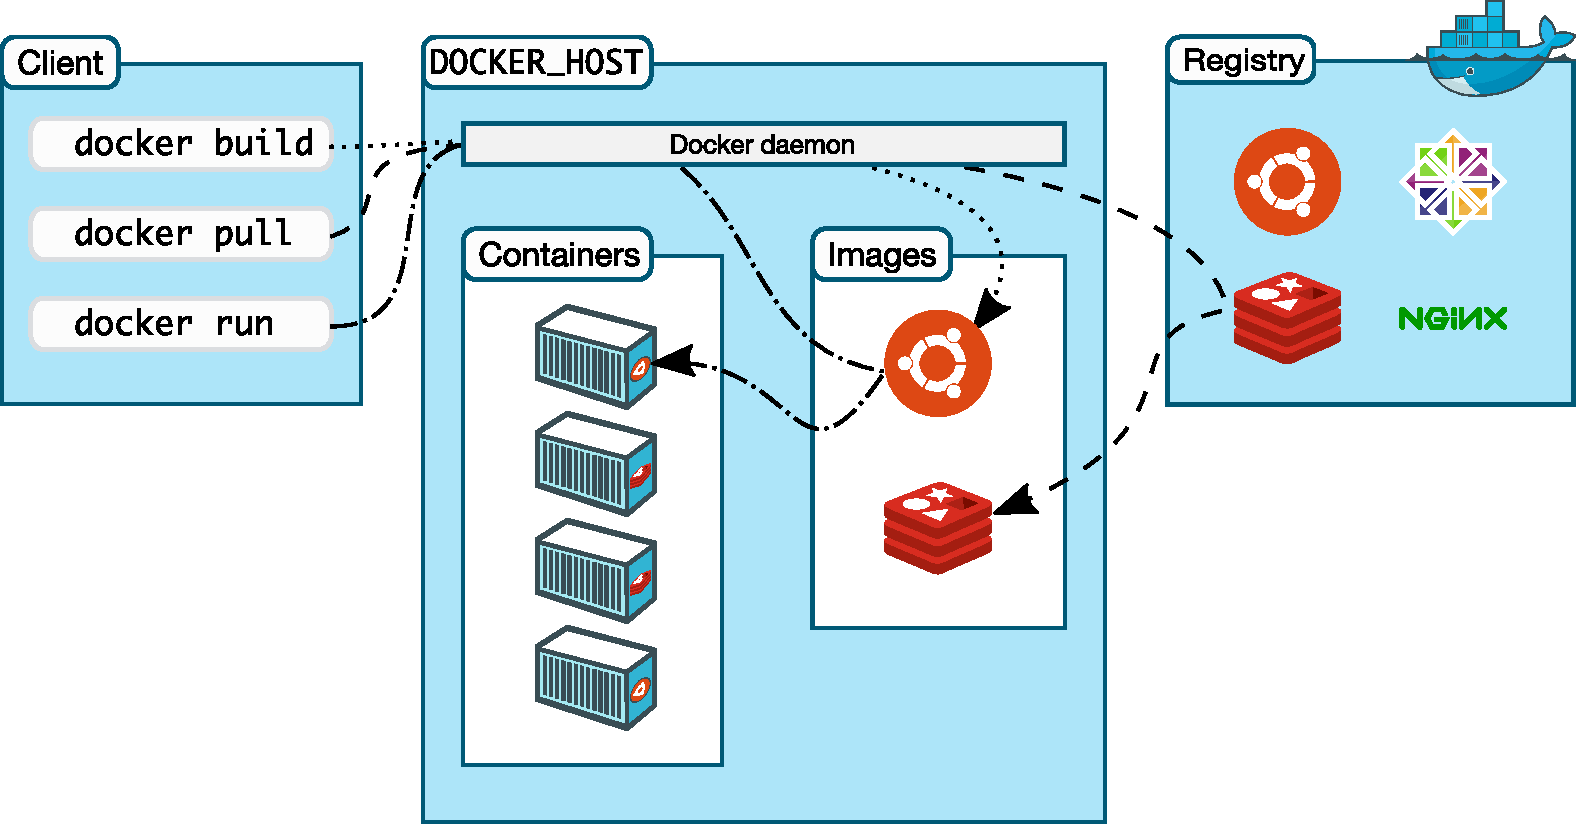
\includegraphics[width=400pt]{immagini/architecture.pdf}
  \caption{Struttura di un container Docker}
\end{center}
\end{figure}
\newpage

\subsection{Cookies} \label{cookieitem}
I cookies rappresentano dei piccoli blocchi di dati, generati lato server e memorizzati sul client, in grado di espletare varie funzioni.
Nella loro configurazione \`e possibile definire diversi attributi a seconda dello scopo di utilizzo degli stessi.

La diversificazione nel loro impiego, identifica diverse tipologie di cookies: 
\begin{itemize}
    \item \textbf{Cookie di sessione}: vengono generati nel momento in cui l'utente effettua operazioni di navigazione web, scadono una volta che viene chiuso il browser.
    \item \textbf{Cookie persistenti}: basano il loro funzionamento su uno specifico arco temporale. In particolare vengono memorizzati lato client e trasmessi nel caso in cui si ha la necessit\`a del loro impiego in un determinato sito web. Una volta terminato il periodo di validit\`a scadono e devono essere generati nuovamente.
    Questa tipologia di cookie viene adottata dai siti web in cui \`e presente un form di autenticazione, mantenendo in questo modo il login.
    \item \textbf{Cookie di terze parti}: tracciano l'attivit\`a dell'utente attraverso la navigazione nei siti web. Vengono impiegati in ambito pubblicitario e generano il collegamento a server differenti da quello in cui si sta fruendo un determinato servizio, per recuperare informazioni memorizzate durante tutta la sessione di navigazione. 
\end{itemize}
L'utilizzo dei cookie, impone una maggiore gestione della sicurezza, soprattutto nella memorizzazione dati relativi a sessioni di login.\cite{kristol2000http}
I cookie di tipologia persistente, vengono impiegati durante l'accesso ai social network;  il salvataggio di questi dati, permette di effettuare login ai servizi, senza l'utilizzo di credenziali.

\subsection{L'ingestione dei dati}
Per Data Ingestion si intende il processo di raccolta dei dati raw (grezzi) dalla loro sorgente e del trasporto e la centralizzazione verso il sistema target.\cite{meehan2017data}

Viene definito anche ETL (Extract/Transform/Load) ovvero estrazione, trasformazione e caricamento. Le tre fasi funzionali assolvono i seguenti compiti:
\begin{itemize}
    \item \textbf{Estrazione}: la prima fase attua le tecniche definite al Capitolo \ref{chap:stato_arte}. Le soluzioni adottate per l'elusione dei controlli e la mitigazione del contrasto saranno dettagliate al Paragrafo \ref{contrasto_scraping}. 
    \item \textbf{Trasformazione}: la seconda fase  si occupa del controllo e del data cleaning, ovvero il processo in grado di garantire l'affidabilit\`a dei dati, anche trasformandoli in formati idoeni al loro utilizzo. Nel caso del progetto di tesi \`e stato scelto il formato JSON, dettagliato al Paragrafo \ref{formato dati}.
    \item \textbf{Caricamento}: la terza e ultima ultima fase rappresenta il caricamento dei dati nel sistema di Big Data Analytics. La gestione di questo step \`e garantita attraverso l'omogeneit\`a negli output e nelle tecnologie richieste dal target per ogni connettore.
\end{itemize}


\subsection{Big Data Analytics}
Con il termine Big Data si definisce un sistema avente tre attributi: grande volume di dati, variet\`a e velocit\`a. 
Il volume rappresenta l'attributo principale, seguito dall'eterogeneità e dalla frequenza di generazione e rilascio dei dati.

L'applicazione del termine ``Big Data Analytics'' comprende tecniche avanzate di analisi dei dati su set di Big Data.\cite{russom2011big}
L'analisi dei dati si distingue a seconda degli strumenti e dei modelli di gestione in tre tipologie:
\begin{itemize}
    \item \textbf{Analisi descrittiva}: descrizione storica e confronto dei dati presenti. Tecnica da impiegare per la catalogazione delle informazioni attuali e passate. 
    \item \textbf{Analisi predittiva}: applicazione di modelli predittivi sui dati, in grado di estrarre e prevedere casi futuri. 
    \item \textbf{Analisi prescrittiva}: propone soluzione automatizzate ed implicazioni di azioni in corso sui dati.
\end{itemize}
L'insieme dei tre modelli di analisi sono applicabili per lo scopo del progetto ed il conseguente studio delle informazioni pubbliche estratte dai social.
\section{Soluzioni al contrasto dello scraping}\label{contrasto_scraping}
\subsection{Generalit\`a}
Le metodologie attuate dalle piattaforme social per contrastare l'attivit\`a di scraping sono state elencate e descritte al Paragrafo \ref{metodi_contrasto}. Si presentano di seguito soluzioni ideali per garantire il funzionamento di un'applicazione resiliente ed in grado di offrire l'estrazione della maggiore quantit\`a di dati.

%%%%%%%%%%%%%%%%%%%%%%%%%%%%%%%%%%%%%%%%%%%%%%%%%%%%%
%aggiungere

\subsection{Gestione degli account} \label{account}
I social network, per la normale attivit\`a sulle loro piattaforme, obbligano ad effettuare la registrazione ed il conseguente login. Le possibilit\`a di accesso ai servizi senza alcuna tipologia di autenticazione sono molto limitate e non giovano in alcun modo ad una completa estrazione dati. Da ci\`o ne consegue la necessit\`a di autenticarsi ai servizi e la creazione di un pool di account. 
L'idoneit\`a di un account risulta essere oggetto di attenzione dai servizi web dei social. Le soluzioni di sicurezza ``anti-bot''\footnote{Con il termine ``bot'' si fa riferimento ad un servizio che compie azioni in modo automatico} sono in grado di individuare la generazione di utenti falsi, definiti ``fake accounts'' promuovendo ed attuando il loro ban.
\subsection{Rotazione dei Cookies}\label{cookie rotation}
Una volta avuta la disponibilit\`a di un numero cospicuo di account validi, si procede con l'azione di login e la successiva estrazione dei cookie, per ogni utenza.
L'estrazione dei cookie pu\`o avvenire attraverso l'accesso diretto dal tool di scraping, oppure tramite lo sviluppo di azioni in funzione di applicazioni di browser automation. 
La seconda opzione risulta essere maggiormente indicata, soprattutto in visione della scadenza di validit\`a temporale dei singoli cookie, che rende obbligatoria la ripetizione del login. 

Un recupero della sessione automatico e il conseguente aggiornamento dei cookie consente la validit\`a continua degli stessi.
Una soluzione implementativa idonea all'elusione del controllo sullo scraping \`e l'introduzione, dopo aver memorizzato tutti i cookie validi degli account, di un sistema di rotazione random sulla selezione ed impiego del cookie appartenente ad un determinato utente.
Questa operazione consente di diversificare gli accessi automatici al social, limitando fortemente la probabilit\`a di ban di un account, osservato che lo stesso verr\`a impiegato per una singola operazione alla volta e successivamente sostituito da un altro nell'elenco, diminuendo cos\`i l'esposizione del singolo.

Ne consegue che un maggior numero di account validi disponibili per l'accesso al social network, consente una massimizzazione dell'elusione al controllo sul singolo utente e la sua attivit\`a.
Avendo pi\`u cookie in grado di essere selezionati dalla funzione random, viene aumentata l'operativit\`a continua, in senso temporale, dell'estrazione dei dati.  

\begin{figure}[!htb]
  \begin{center}
  \includesvg[width=425pt]{immagini/cookie_rotation.svg}
  \caption{Cookie Rotation}
\end{center}
\end{figure}
\newpage

\subsection{Latenza}
Il contrasto alle soluzioni anti-scraping richiede anche un tempo operativo pi\`u dilatato. Si rende necessaria l'aggiunta di latenza tra le operazioni in termini di secondi o minuti, garantendo un profilo di attivit\`a non sospettoso.
L'aggiunta di tempo d'attesa tra le operazioni consente la simulazione dell'attivit\`a umana sulla piattaforma web, non dimostrando l'automaticit\`a e la velocit\`a tipica dei bot.
Un'idea implementativa \`e l'introduzione di attesa random nell'ordine dei minuti. Alcuni tool di scraping prevedono automaticamente una funzione di salvaguardia dell'account, bloccando le richieste ed azionando un'attesa a seconda dell'onerosit\`a dell'attivit\`a da svolgere.
Considerato che l'obiettivo del progetto \`e la garanzia operativa senza l'effettiva necessit\`a di velocit\`a nella produzione dei dati, il ritardo tra le azioni non vincola l'impiego del software da produrre.

\subsection{User Agent}
Lo user agent identifica un campo del protocollo HTTP in cui vengono dichiarate delle informazioni relative al dispositivo che si connette al server ed il browser utilizzato.
Un esempio di user agent valido per la connessione ad Instagram e relativo ad un dispositivo mobile iOS \`e il seguente:
\begin{center}
    Mozilla/5.0 (iPhone; CPU iPhone OS 15\_5 like Mac OS X) AppleWebKit/605.1.15 (KHTML, like Gecko) Mobile/15E148 Instagram 244.0.0.12.112 (iPhone12,1; iOS 15\_5; en\_US; en-US; scale=2.00; 828x1792; 383361019)
\end{center}
Nell'atto dello scraping \`e importante definire user agent idonei ed approvati dal servizio target in quanto lo stesso pu\`o effettuare specifici controlli e non accettare le richieste provenienti da user agent non presenti in ``white-list''\footnote{Si fa riferimento all'elenco degli user agent accettati dal servizio.}.
\subsection{Indirizzi IP}\label{ip_rotation}
I sistemi anti-scraping pongono particolare attenzione agli indirizzi IP dai quali provengono le richieste. Come introdotto al Paragrafo \ref{metodi_contrasto}, viene attuato un controllo sulla affidabilit\`a dell'indirizzo da cui si \`e connesso un determinato utente. Nel caso in cui venissero rilevate delle azioni ``insolite'' o massive, si procede con il ban temporaneo o permanente, a seconda delle policy previste dal servizio.

Un'idea implementativa \`e l'utilizzo di un pool di indirizzi IP da proxy condivisi. L'introduzione di una ``ip-rotation'' randomica, seguendo quanto progettato per la cookie-rotation (Paragrafo \ref{cookie rotation}), pu\`o diminuire il numero di ban e garantire un maggiore impiego delle utenze a disposizione.

Si riporta uno schema per il funzionamento di ``ip-rotation''.
\begin{figure}[!htb]
  \begin{center}
  \includesvg[width=425pt]{immagini/ip_rotation.svg}
  \caption{IP Rotation}
\end{center}
\end{figure}
\subsection{Sistemi distribuiti}\label{sistemi_distribuiti}
Un sistema distribuito \`e un insieme di processi indipendenti ed interconnessi che cooperano per la condivisione di risorse. \cite{tanenbaum2007sistemi}

Le caratteristiche dei sistemi distribuiti sono:
\begin{itemize}
    \item \textbf{Openess}: possibilit\`a di estendere, in termini di risorse, un sistema.
    \item \textbf{Concurrency}: presenza di pi\`u processi coesistenti su un'unica risorsa.
    \item \textbf{Scalability}: capacit\`a del sistema di aumentare ed adattarsi all'aumento dimensionale del lavoro da compiere senza alterare la funzionalit\`a.
    \item \textbf{Fault tolerance}: tollerenza del sistema al guasto.
\end{itemize}

%%%%%%%%%%%%%%%%%%%%%%%%%%%%%%%%%%%%%%%%%%%%%%%%%%%%%
%continuare
L'implementazione della distribuzione su un'applicazione di scraping consente di ottenere molteplici vantaggi oltre a quelli propri dei sistemi distribuiti.
Pu\`o essere identificata come una soluzione generalizzata al contrasto dello scraping, in quanto consente di aggiungere funzionalit\`a utili all'elusione dei controlli.
La funzionalit\`a di un sistema distribuito per lo scraping necessita della presenza di un controller in grado di inviare comandi ai singoli nodi e ricevere risposte in termini di dati estratti dai singoli scraper-bot.
La comunicazione tra controller e singoli bot pu\`o avvenire tramite Remote Procedure Call (RPC) \footnote{Indica una procedura avviata su dispositivo diverso da quello sul quale viene eseguito un programma.}
Si presentano di seguito gli schemi di funzionamento e comunicazione delle varie parti in azione durante lo svolgimento di un'attivit\`a di scraping distribuita.

%%%%%%aggiungere info su sistemi distribuiti

%Idea di scraping distribuito con schema 
\begin{figure}[!htb]
  \begin{center}
  \includesvg[width=400pt]{immagini/distributed_scraper.svg}
  \caption{Schema di un'applicazione di scraping distribuita}
\end{center}
\end{figure}

\begin{figure}[!htb]
  \begin{center}
  \includesvg[width=400pt]{immagini/bot_controller.svg}
  \caption{Schema di comunicazione controller-bot}
\end{center}
\end{figure}
%\clearpage
\newpage
\section{Output}
\subsection{Gestione dei dati estratti}
I dati in output devono essere uniformi e pronti all'ingestione in un sistema di analisi. Per garantire l'uniformit\`a si devono individuare formati e tipi di dato uguali, a fronte dell'estrema eterogeneit\`a dei dati raccolti. 
Un esempio \`e l'introduzione dell'utilizzo di UUID (Universally Unique Identifier) per la denominazione dei file e la compressione delle cartelle in formato zip per la riduzione dello spazio di memoria occupato. UUID rappresenta un identificativo univoco universale composto da 128 bite rappresentato da caratteri esadecimali divisi in gruppi.
Si fa presente che i dati effettivamente estratti restano in formati direttamente fruibili quali JSON, JPEG e MP4. L'impiego di UUID e zip ha come obiettivo la sola modifica della denominazione e della dimensione dei file per la loro successiva ingestione ed analisi come Big Data.

Diversi tool offrono la possibilit\`a di individuare file gi\`a presenti in locale, frutto di estrazioni precedenti, evitando di effettuare un nuovo download. Questa funziona viene adottata anche per individuare eventuali cambiamenti ``storici'' nell'account target: nel caso in cui un elemento gi\`a estratto in passato non venga pi\`u selezionato e scaricato, si deduce automaticamente la presenza di un'azione di cancellazione dello stesso dalla piattaforma social.

L'analisi comportamentale del software rispetto a cambiamenti storici nell'output garantisce un elevato numero di informazioni aggiuntive che vanno ad ampliare i metadati gi\`a frutto di estrazione. Le stesse, combinate con il resto, garantiscono una continuit\`a informativa nell'atto dell'ingestione dei dati nel sistema di Big Data Analytics.

Si riporta di seguito uno schema di gestione dei dati di output provenienti dal software di scraping.

\begin{figure}[!htb]
  \begin{center}
  \includesvg[width=400pt]{immagini/output.svg}
  \caption{Schema di gestione dei dati per l'ingestione}
\end{center}
\end{figure}
\newpage

\afterpage{\blankpage}

%Capitolo 4: Caso di studio
\chapter{Il caso di studio} \label{chap:caso_studio}
\section{I social di Meta}
Per il progetto sono stati individuati come obiettivi i due principali social network della societ\`a Meta Platforms Inc.\footnote{\url{https://about.meta.com}}, ovvero Facebook ed Instagram. 
Le due piattaforme sono state selezionate principalmente per il vasto pubblico attivo e conseguentemente per la quantit\`a di informazioni online.
\subsection{Facebook}
Facebook, nato nel 2004, conta ad oggi secondo i dati ufficiali rilasciati dalla societ\`a, 2.93 miliardi di utenti attivi  \footnote{\url{https://investor.fb.com/investor-news/press-release-details/2022/Meta-Reports-Third-Quarter-2022-Results/default.aspx}}. Il social permette di condividere informazioni testuali e multimediali sia pubblicamente che privatamente, attraverso singole pagine personali, pagine pubbliche e gruppi. 
La funzionalit\`a denominata come ``amicizia'' consente la creazione di una rete sociale per ogni singolo utente. 
Le foto, i video, i post, le storie, le reazioni, i commenti, la condivisione di contenuti in diretta, la presenza di un market ed i messaggi istantanei sono i principali punti di forza della piattaforma.
L'imponente diffusione di questo social ha implicato l'impiego dello stesso anche come strumento informativo ufficiale da parte di organi statali, di stampa e di informazione pubblica.
L'aggiornamento costante del servizio aggiunge continuamente nuove funzionalit\`a che vanno ad ampliare la quantit\`a di informazioni pubblicate.

\subsection{Instagram}
Instagram, pubblicata nel 2010, raggiunge ad oggi quasi lo stesso numero di utenti attivi di Facebook. I punti di forza di questo social, nato inizialmente per condividere solamente foto, riuniscono varie possibilit\`a di pubblicazione di informazioni online. Oltre alle semplici foto, possono essere pubblicati altre tipologie di contenuti multimediali come video e musica. La piattaforma consente la pubblicazione dei media sotto forma di post, permettendo agli utenti di cliccare ``mi piace'' e scrivere commenti. Inoltre il singolo utilizzatore pu\`o generare la sua rete sociale tramite il ``follow'' lett. ``seguire'' ed attraversp l'utilizzo il sistema di messaggistica istantanea e la condivisione di storie e post.
I profili degli utenti possono essere impostati come pubblici o privati, questi ultimi necessitano l'autorizzazione del proprietario per essere consultati.
Anche nel caso di Instagram, l'aggiornamento \`e costante in quanto vengono rilasciate costantemente nuove funzionalit\`a a favore degli utenti.


\subsection{Termini e condizioni}
Le piattaforme sopra introdotte individuano termini e condizioni d'utilizzo simili. Nel particolare, in riferimento alla finalit\`a del progetto sviluppato, viene esplicitamente vietato qualsiasi comportamento riconducibile ad azioni di web scraping o pi\`u in generale di collezione dei dati in maniera automatica.\cite{doi:10.1177/2056305120940703}
Come riportato dal file ``robots.txt''\footnote{\url{https://instagram.com/robots.txt}} di Facebook:
\begin{center}
    \textit{``Notice: Collection of data on Facebook through automated means is prohibited unless you have express written permission from Facebook and may only be conducted for the limited purpose contained in said permission. See: \url{http://www.facebook.com/apps/site_scraping_tos_terms.php}''}
\end{center}
Meta contrasta la External Data Misuse (EDM)\footnote{Uso improprio ed esterno dei dati.} promuovendo nuove tecniche contro lo scraping dei dati.
Un deterrente attuato dalla societ\`a \`e anche la promozione di azioni legali contro attivit\`a non consentite dai termini di servizio. Pubblicando notizie ed aggiornamenti su come viene contrastata la collezione automatica di dati si punta a dissuadere un eventuale soggetto interessato all'attivit\`a.
%%%%%%%%%%%%%%%%%%%%%%%%%%%%%%%%%%%%%%%%%%%%%%%%%%%%%%%%continuare


\section{Strumenti Open Source per lo scraping}
Il funzionamento dei singoli connettori di scraping si basa su due tool open source individuati come migliori per lo scopo designato. In particolare, per i due social network oggetto di studio, Facebook e Instagram, si \`e fatto uso rispettivamente di ``facebook-scraper''\footnote{\url{https://pypi.org/project/facebook-scraper/}} e ``instaloader''\footnote{\url{https://instaloader.github.io/}}.

L'individuazione e lo studio di questi strumenti, si \`e basato su un attento confronto delle loro caratteristiche tecniche e di funzionamento.
I due tool utilizzati non impiegano le API ufficiali rilasciate dai rispettivi social. Ci\`o avviene a causa della forte limitazione all'estrazione dati che viene imposta, nel caso specifico da Facebook e Instagram. 

Questa limitazione rende necessario ricorrere a soluzioni che contrastano le linee guida definite dai fornitori dei servizi social, adottando tecniche in grado di eludere i controlli messi in campo e giungere all'obiettivo del progetto garantendo efficienza.

Le piattaforme social vengono continuamente sottoposte a nuovi sviluppi ed aggiornamenti, causando ovvi problemi all'operativit\`a degli strumenti scelti. Ne consegue un continuo aggiornamento dei tool ed una attenta ricerca per la  gestione tecnica del loro funzionamento.

\section{Soluzioni implementative per Facebook}
\subsection{Estrazione e formato dei dati}
Il connettore di Facebook basa il suo funzionamento sul progetto ``facebook-scraper''.
L'acquisizione e la gestione dei dati estratti da questo social network, sono state effettuate con l'obiettivo di essere rese fruibili da parte di sistemi di analisi dati (Big Data Analytics).
Il tool opera direttamente effettuando richieste GET sulle diverse estensioni dei link, a partire da un target\footnote{Si fa riferimento all'obiettivo dell'attivit\`a di scraping.} dato in input.
Nel caso specifico, il route\footnote{Si fa riferimento al percorso definito dal link relativo.} definito dall'API genera l'input per le singole funzioni dello scraper, avviando il processo di identificazione del target e conseguente iterazione sulla gerarchia di link collegati ad esso, ricavando i dati richiesti.
Sono state definite in totale tre route o ``cammini'' per le API, rispettivamente per lo scraping di profili, pagine e gruppi.

Un esempio di route per l'estrazione di tutti i dati di un profilo \`e:
\begin{center}
    localhost:5000/profile/{username}/posts
\end{center}
I dettagli relativi alle singole funzioni sviluppate sono:
\begin{itemize}
    \item \textbf{Profili}: in ``profile.py'' vengono descritte tutte le funzioni per lo scraping di profili pubblici e privati. In particolare si ha la possibilit\`a di scaricare le informazioni generali di un profilo ed anche tutti i post, le foto ed i video, con relativi commenti e reazioni. 
    La funzione ``get\_posts`` di facebook-scraper restituisce un JSON contenente una moltitudine di informazioni da processare. Di conseguenza sono state sviluppate funzioni in grado di elaborare il file JSON ed estrarre ci\`o di interesse.
    Per le foto, osservato che Facebook prevede la presenza di foto in bassa qualit\`a (identificate come anteprime) e foto in alta qualit\`a (identificate come foto dei post) si \`e provveduto a differenziare il download di questi media in funzioni differenti.
    Si riporta in Appendice al paragrafo \ref{scraping_funzioni} il codice per il download dei post e dei media da un profilo.
    \item \textbf{Pagine}: in ``pages.py'' vengono descritte le funzioni per lo scraping di pagine. Come descritto per i profili, anche in questo caso si ha la possibilit\`a sia di estrarre le informazioni generali di una pagine, che i relativi post con media, commenti e reazioni.
    \item \textbf{Gruppi}: in ``groups.py'' sono definite le funzioni per lo scraping di gruppi pubblici e privati. Per i gruppi pubblici valgono le stesse modalit\`a descritte per profili e pagine, mentre per i gruppi i privati lo scraping \`e limitato solo all'estrazioni di informazioni generali e delle indicazioni sugli amministratori. Lo scraping completo di un gruppo privato pu\`o essere effettuato solamente se l'account (ed i relativi cookies) utilizzato per lo scraping risulta appartente al gruppo.
\end{itemize}
Facebook-scraper \`e stato selezionato come migliore servizio da integrare nel funzionamento del connettore di dati dal social Facebook. Il confronto con gli altri tool validi individuati \`e riportato in Tabella \ref{tabella_fb}.

I dati raccolti attraverso l'integrazione di questo tool sono stati sottoposti ad una precisa organizzazione come descritto nel paragrafo \ref{formato dati}.
L'insieme delle qualit\`a descritte in Tabella \ref{tabella_fb} fanno si che facebook-scraper garantisca un'operativit\`a continua nell'estrazione delle informazioni.
In particolare la possibilit\`a di gestione del tempo nelle richieste effettuate consente di simulare la normale attivit\`a di interazione umana con il servizio web, evitando il riconoscimento di automazione con conseguente ban.
Gli ulteriori accorgimenti relativi alle tecniche di elusione dei controlli sono descritti al Paragrafo \ref{contrasto_scraping}.

%\newpage
\begin{table}[!htb]
\centering
\caption{Confronto Tool per Scraping di Facebook.}
\label{tabella_fb}
\begin{tabular}{|p{4,5cm}|p{4,5cm}|p{4,5cm}|}
\hline
\textbf{FACEBOOK-SCRAPER} & \textbf{FACEBOOK-POST-SCRAPER-SELENIUM} & \textbf{FACEBOOK-SCRAPER-SELENIUM} \\\hline
 No API         &  No API                &   No API                        \\\hline
Login non obbligatorio &   Login obbligatorio & Login obbligatorio  \\\hline
Mantenimento di sessione di login & - & - \\\hline
Gestione dei cookies sia in formato NETSCAPE che in formato JSON & - & - \\\hline
Download anonimo completo di profili pubblici e privati & Download anonimo dei soli post di profili pubblici, privati & Download anonimo del solo testo dei post di profili pubblici e privati\\\hline
Download di hashtag, commenti, tag geografici e descrizioni per ogni post & Download di commenti per ogni post (con foto e link) & - \\\hline
Download di tutte le reazioni per ogni post & Download di solo tre reazioni per post & -\\\hline
Download anonimo completo di pagine & Download anonimo dei post delle pagine & Download anonimo dei post delle pagine \\\hline
Download anonimo di gruppi pubblici e privati & - & Download dei post dei gruppi pubblici e privati \\\hline
Download di file JSON & Download di file JSON & Download di file CSV\\\hline
I media vengono estratti tramite metodo GET & I media vengono estratti tramite metodo GET & -\\\hline
\end{tabular}
\end{table}
\begin{table}[!htb]
\begin{tabular}{|p{4,5cm}|p{4,5cm}|p{4,5cm}|}
\hline
Personalizzazione di filtri di ricerca & - & -\\\hline
- & Utilizzo di ``Selenium'' & Utilizzo di ``Selenium'' \\\hline
Download in elenco degli amici & - & - \\\hline
Il download di profili privati avviene solo se l’account usato fa parte della lista degli amici dall’account target & Il download di profili privati avviene solo se l’account usato fa parte della lista degli amici dall’account target & Il download di profili privati avviene solo se l’account usato fa parte della lista degli amici dall’account target \\\hline
Orientato al solo scraping di profili di terzi & Orientato al solo scraping di profili di terzi & Orientato al solo scraping di profili di terzi \\\hline
\end{tabular}
\end{table}
\newpage


\subsection{Risoluzione del contrasto}
Durante il funzionamento del tool, si incorre facilmente in errori dovuti alle soluzioni anti-scraping. In particolare si ricevono i seguenti codici di stato\footnote{Codici di stato HTTP, indicano l'esito di una comunicazione HTTP} e comunicazioni:
\begin{itemize}
    \item \textbf{429 Too Many Requests}: il codice di stato 409 viene presentato quanto viene superato il limite di richieste da parte di un indirizzo IP in un determinato arco temporale. Una volta presente questo codice, sar\`a necessario riavviare il processo di scraping.
    \item \textbf{Temporary Ban}: errore presentato quando \`e stata individuata un'attivit\`a sospetta da parte di un account. Da test effettuati, il ban temporaneo di un profilo dura 24/48 ore, successivamente torna ad essere operativo.
    \item \textbf{Account disabled}: qualora un account sottoposto a un ban temporaneo continui ad effettuare richieste, viene presentato l'errore e la comunicazione di ban permanente a causa dell'attivit\`a non consentita. L'account non risulter\`a essere pi\`u recuperabile.
    \item \textbf{Unusual Activity}: avviso di attivit\`a sospetta proveniente da un account. Viene bloccata l'attivit\`a in corso senza ulteriori ``provvedimenti''. Nel caso in cui lo stesso account, con lo stesso IP, continui operazioni di tipo massivo, si incorrer\`a in modo certo a un ban temporaneo.
\end{itemize}
Per limitare la comparsa degli errori sopra riportati \`e stato sviluppato un sistema di rotazione dei cookies, come presentato al paragrafo \ref{cookie rotation}.

I cookie all'interno del progetto sono stati gestiti ed utilizzati per il login degli account utilizzati per lo scraping. La gestione si \`e basata sulla estrazione e memorizzazione dei valori necessari per il funzionamento dei tool scelti.

Per estrarre i cookie relativi alla sessione dei singoli account si \`e fatto uso di Selenium, grazie al quale, automatizzando le operazioni su browser Chromium in modalit\`a headless, si sono potuti estrarre i valori dei cookie di interesse per il login.

Si riporta il codice relativo all'implementazione di Selenium ed un esempio dei valori dei cookie estratti in Appendice \ref{cookie_code}.

La funzione ``cookie\_rotation'' ha consentito il mantenimento di una continuit\`a operativa del tool, grazie all'elusione dei controlli.
Si riporta il codice della funzione:
\inputminted[bgcolor=bg]{python}{codice/cookie_rotation_fb.txt}

Oltre alla soluzioni adottata sui cookie, si \`e prevista per ogni azione di download con richieste dirette al server target, l'aggiunta di tempi d'attesa nell'ordine dei secondi. Rallentando l'attivit\`a si \`e aumentata la resistenza del tool contro eventuali azioni di ban, immedesimando l'utilizzo del social da parte di un umano, inteso come utente reale e non bot.
\begin{center}
\begin{minted}[bgcolor=bg]{python}
time.sleep(15)
\end{minted}
\end{center}
La funzione ``time.sleep'' in Python, sospende l'esecuzione di un determinato processo sulla base del numero di secondi inseriti in input.

Tutte le funzioni elencate necessitano di login con account validi. La gestione degli account avviene attraverso la memorizzazione delle credenziali in file JSON, dal quale vengono estratte per avviare i processi di login.
\subsection{Aggiornamenti}
A causa dell'attivo e consistente contrasto ed all'aggiornamento tecnico delle infrastutture dei social, durante lo sviluppo si sono presentate diverse problematiche relative al corretto funzionamento dello scraping.
Ogni questione \`e stata prontamente risolta grazie al rilascio di nuove versioni del tool.
La cronistoria dei rilasci \`e presente nello schema riportato al paragrafo \ref{confronti_software}.

\section{Soluzioni implementative per Instagram}
\subsection{Estrazione e formato dei dati}
Il connettore di Instagram basa il suo funzionamento sul progetto ``instaloader''.
Instaloader consente il download di profili completi di media (foto e video) e metadati\footnote{Serie di informazioni aggiuntive sui dati.} per ogni post.
L'acquisizione e la gestione dei dati estratti da questo social network, sono state effettuate con l'obiettivo di essere rese fruibili da parte di sistemi di analisi dati (Big Data Analytics). 

Instaloader \`e stato selezionato dopo la comparazione del suo funzionamento con altri tool open source individuati. Il confronto \`e riportato in Tabella \ref{tabella_insta}.
L'attivit\`a effettuata con instaloader ha subito una organizzazione e gestione simile a quella di facebook-scraper.
Le principali differenze, riguardanti l'approccio di funzionamento del tool, sono state uniformate con particolare attenzione alla gestione dei dati in output.

Lo sviluppo dell'API prevede la presenza di route, le quali generano l'input per le singole funzioni dello scraper, avviando l'iterazione sulla gerarchia di link collegati al target, ricavando i dati richiesti.
Un esempio di route per l'estrazione dei post con il connettore di Instagram \`e:
\begin{center}
    \url{localhost:5000/<username>}
\end{center}

Anche nel caso di Instagram, le attivit\`a messe in campo per l'elusione dei controlli anti-scraping sono descritte al Paragrafo \ref{contrasto_scraping}.

Le principali funzioni sviluppate ed impiegate per lo scraping di questo social sono:
\begin{itemize}
    \item \textbf{Post, foto e video}: la funzione ``profile\_dl'' consente di estrarre tutti i post di un profilo pubblico senza effettuare il login e tutti i post di un profilo privato se si effettua il login e se l'account in uso fa parte dei follower approvati dal target. \`E possibile anche effettuare il download dei post in cui l'obiettivo \`e stato taggato. La funzione prevede un controllo della frequenza delle richieste, limitando il numero delle stesse ed aggiungendo ritardo nell'ordine dei secondi. Insieme ai media relativi a tutti i post viene memorizzata anche la foto profilo dell'account.
    Per ogni post estratto, viene memorizzato anche un file JSON contenente informazioni aggiuntive come i commenti, il numero di mi piace, l'eventuale posizione GPS, la data e l'ora di pubblicazione, le informazioni del profilo, eventuale connessione del profilo con un account Facebook ed altri metadati. 
    \item \textbf{Storie}: la funzione ``stories\_dl'' consente di estrarre tutte le storie valide\footnote{Per validit\`a di una storia si fa riferimento, secondo le policy di Instagram, al contenuto pubblicato entro le 24 ore dalla visione.} pubblicate da un utente. La funzione necessita di login al social e prevede il controllo della frequenza. 
    \item \textbf{Followers e seguiti}: le funzioni ``followers\_dl'' e ``followee\_dl'' prevedono la possibilit\`a di restituire in output elenchi in JSON dei follower e dei seguiti dell'account target. Necessitano di login e sono molto vulnerabili alle azioni di contrasto. La loro vulnerabilit\`a nasce dal numero di elementi da estrarre. Nella maggioranza dei casi, il numero di follower o di seguiti \`e maggiore rispetto al numero di post pubblicati ed appartenente all'ordine delle centinaia o migliaia. Ne consegue che il numero di richieste segue il numero di elementi, esponendo l'azione al controllo.
    \item \textbf{Geolocalizzazione}: la funzione ``location\_dl'' consente, a partire dall'input di un luogo, di effettuare l'estrazione di tutti i post geolocalizzati in quel punto. Ne consegue che questa funzione rappresenta un'estensione rispetto al normale download dei post da un profilo, in quanto estende la possibilit\`a di ricerca sulla base della posizione.
\end{itemize}
Il tool offre la possibilit\`a di analizzare il comportamento storico di un utente, confrontando i dati gi\`a scaricati e memorizzati rispetto ad una nuova azione di scraping. Ci\`o oltre ad evitare ridondanza, consente anche di ottimizzare le richieste al server, riducendone il numero.

Anche in questo caso, tutte le funzioni elencate che necessitano di login con account validi, gestiscono le credenziali attraverso file JSON, dal quale vengono estratte per avviare i processi.

Tutti i media vengono memorizzati nella qualit\`a massima, ovvero la stessa presente alla normale fruizione dei dati dal social. 
Si riportano in Appendice al Paragrafo \ref{scraping_funzioni_insta} le funzioni di scraping adottate per lo sviluppo del connettore.
%\newpage
\clearpage
\begin{table}[!htb]
\centering
\caption{Confronto Tool per Scraping di Instagram.}
\label{tabella_insta}
\begin{tabular}{|p{4,5cm}|p{4,5cm}|p{4,5cm}|}
\hline
\textbf{INSTALOADER} & \textbf{INSTAGRAPI} & \textbf{INSTAGRAM-SCRAPER-2021-SELENIUM} \\\hline
No API & Basato su API ufficiale di Instagram & No API \\\hline
Login obbligatorio per alcune azioni & Login obbligatorio & Login obbligatorio\\\hline
Supporto autenticazione a due fattori & Supporto autenticazione a due fattori & Supporto autenticazione a due fattori \\\hline
Download anonimo di profili pubblici e privati & Download anonimo di profili pubblici, privati & Download anonimo di profili pubblici, privati \\\hline
Il download di profili privati avviene solo se l’account usato fa parte della lista dei follower dell’account target & Il download di profili privati avviene solo se l’account usato fa parte della lista dei follower dell’account target & Il download di profili privati avviene solo se l’account usato fa parte della lista dei follower dell’account target \\\hline
Download di storie, mi piace, commenti e tag geografici & Download di storie, mi piace, commenti e tag geografici & -\\\hline
Download diretto di foto e video & - & - \\\hline
Download dei file in JPG, MP4 e JSON & Download di file JSON & Download di file JSON \\\hline
- & - & Utilizzo di Selenium \\\hline
Rilevazione di cambio di username & - & -\\\hline
Rilevazione dei post eliminati & - & - \\\hline
\end{tabular}
\end{table}
\clearpage
\begin{table}[!htb]
\begin{tabular}{|p{4,5cm}|p{4,5cm}|p{4,5cm}|}
\hline
Download di metadati aggiuntivi & - & -\\\hline
Personalizzazione di filtri di ricerca & - & - \\\hline
Mantenimento di sessione di login & - & - \\\hline
Permette il download di post appartenenti ad uno specifico periodo temporale & - & -\\\hline
Rilevazione automatica e continuazione di download interrotti & - & - \\\hline
- & Challenge resolver (per verification code login su email e sms) & - \\\hline
Presenza di buon supporto da parte della community & - & - \\\hline
\end{tabular}

\end{table}


\subsection{Risoluzione del contrasto} \label{risoluzione_insta}
Come per il tool di Facebook, anche per lo scraping di Instagram, si presentano errori dovuti alle soluzioni anti-scraping:
\begin{itemize}
      \item \textbf{429 Too Many Requests}: il codice di stato 429 viene presentato quanto viene superato il limite di richieste da parte di un indirizzo IP in un determinato arco temporale. Una volta presente questo codice, sar\`a necessario riavviare il processo di scraping.
      \item \textbf{401 Unauthorized}: il codice 401 viene presentato quando si tenta di effettuare il download di dati da profili privati o senza aver effettuato il login al servizio.
      \item \textbf{Ban}: diversamente da quanto accade con Facebook in cui \`e presente anche un soft-ban, per Instagram il ban di un profilo risulta essere definitivo in caso di azioni non consentite. Ci\`o avviene con pi\`u frequenza quando ad le azioni non riconosciute sono effettuate da un account appena creato. Lo studio e lo sviluppo del connettore ha evidenziato come Instagram attui una politica di controllo nei confronti di account appena creati, attenzionando e limitando il numero di operazioni consentite.
      \item \textbf{Riconoscimento ``umano'' anti-bot}: una volta che un account \`e stato segnalato a causa di azioni sospette, viene richiesta l'identificazione personale del soggetto per eliminare eventuali bot. Nel caso in cui ci\`o non avvenisse, il profilo verr\`a sottoposto a ban permanente. Si riporta schermata di richiesta fotografia ``selfie'' con specifiche azioni da effettuare per il riconoscimento dell'utente in qualit\`a di persona fisica proprietaria dell'account.

\end{itemize}
  \begin{figure}[!htb]
          \centering
          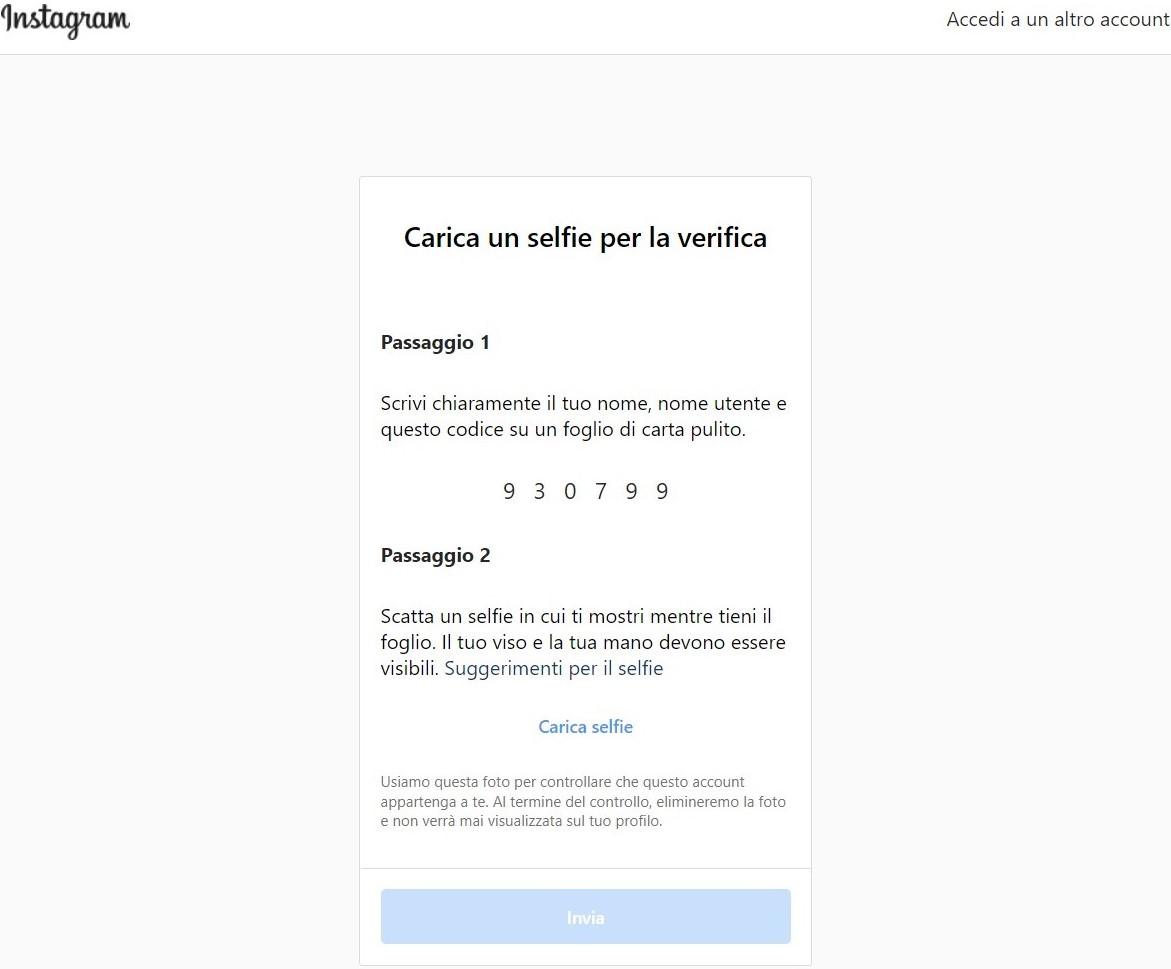
\includegraphics[width=400pt]{immagini/login_selfie.jpg}
    \end{figure}
\newpage

Lo studio e lo sviluppo di tecniche di elusione dei controlli e del contrasto sopra descritto si \`e attuato adottando le stesse idee implementative del connettore di Facebook.

In questo caso, come fatto per la funzione ``cookie\_rotation``, osservando la diversa gestione dei cookie da parte del tool per il connettore di Instagram, si \`e sviluppata una funzione di ``account\_rotation'' di cui si riporta il codice.

\inputminted[bgcolor=bg]{python}{codice/account_rotation_insta.txt}

\subsection{Aggiornamenti}
Come descritto per il connettore di Facebook, le problematiche di sviluppo del connettore e di impiego del tool instaloader sono state causate, oltre che dalle soluzioni anti-scraping, dagli aggiornamenti della piattaforma.
Le maggiori difficolt\`a affrontate nello sviluppo hanno riguardato la gestione del login al servizio, continuamente aggiornata da Instagram sia in termini di funzionalit\`a che in termini di sicurezza.

Al Paragrafo \ref{confronti_software} viene presentata la cronistoria degli aggiornamenti del tool su cui si basa il connettore.
\section{Tecnologie utilizzate} \label{tecnologie_utilizzate}
Le soluzioni tecniche adottate per lo sviluppo di questo progetto sono state basate sul concetto di portabilit\`a e operativit\`a continua del servizio di raccolta dati. 

Il linguaggio scelto per lo sviluppo del progetto \`e stato Python\footnote{\url{https://www.python.org/}}, il quale grazie alla vasta offerta di librerie e strumenti dedicati, \`e risultato essere idoneo ad applicazioni di Web Scraping e di analisi ed elaborazione dati.
Inoltre Python si presenta come uno strumento vantaggioso per lo sviluppo di API\footnote{Application Programming Interface.}, fondamentali per permettere il riuso del codice e garantire un utilizzo e un'inclusione delle funzionalit\`a da parte di altri sviluppatori. 

Le scelte tecnologiche adottate sono state definite tramite l'impiego di strumenti Open Source, di formati dati universali e leggibili e di paradigmi architetturali per lo sviluppo web.

Lo sviluppo e l'impiego di software container, ha permesso di massimizzare la portabilit\`a del servizio, garantendo uniformit\`a e produttivit\`a.

L'individuazione di tool open source si \`e basata su uno studio e confronto delle carattistiche, ponendo attenzione anche all'attivit\`a e al seguito delle community di sviluppatori, in modo tale da garantire continuit\`a e costanza nell'aggiornamento dei servizi.

\subsection{Formato dei dati}\label{formato dati}

Lo standard individuato per la gestione dei dati estratti \`e il formato JSON.

JSON \`e un formato di testo per la serializzazione di dati strutturati basato sul linguaggio di programmazione JavaScript, dal quale per\`o non dipende.
JSON rappresenta quattro tipi di dato fondamentali (stringhe, numeri, valori booleani e nulli) e due tipi strutturati (oggetti e vettori).\cite{bray2014javascript}
Grazie alla sua chiara sintassi, rappresenta uno standard interpretabile facilmente sia da persone che da macchine garantendo portabilit\`a e interoperabilit\`a multipiattaforma, fondamentale per l'impiego delle API sviluppate in questo progetto.

L'alta leggibilit\`a del formato JSON ha permesso una manipolazione dei file di output, garantendo soluzioni tecniche idonee per la successiva estrazione dei dati.

La successiva soluzione per il salvataggio dei dati richiesti si basa su formati standard di file multimediali come MP4 e JPG. Essendo lo scraping massivo di dati e la conseguente ingestione in sistemi di analisi dati l'obiettivo finale del progetto, si \`e reso necessario comprimere tutti i dati raccolti in formato ZIP.

Il formato ZIP \cite{zip} è un formato di compressione dati senza perdita di informazioni in grado di ridurre lo spazio occupato dai file.
L'utilit\`a della compressione dei file si rende fondamentale nel processo di ingestione dei dati in sistemi di Big Data Analytics.



\subsection{API}

Il progetto si \`e basato sullo sviluppo di API RESTful utilizzando il servizio Flask\footnote{\url{https://flask.palletsprojects.com/en/2.2.x}}.

Flask \`e un framework per applicazioni web, caratterizzato dalla sua leggerezza ed ampia compatibilit\`a. Offre scalabilit\`a e gestione di progetti complessi, non richiedendo specifici strumenti o scelte progettuali; in questo modo vengono favorite le opzioni implementative delineate dello sviluppatore.
Le funzionalit\`a di Flask impiegano due dipendenze: Werkzeug\footnote{\url{https://werkzeug.palletsprojects.com/en/2.2.x}} e Jinja2\footnote{\url{https://jinja.palletsprojects.com/en/3.1.x}}.
Werkzeug gestisce le attivit\`a di routing, debugging ed il protocollo di trasmissione WSGI\footnote{Web Server Gateway Interface.}, mentre Jinja2 gestisce i template per le API.
Lo sviluppo di API REST tramite Flask consente di instanziare le singole applicazioni, associando singoli route (percorsi) alle varie funzioni, sotto forma di URL.
La risposta alle varie richieste, fornita dal server, fornisce in aggiunta un HTTP Response (codice) che, a seconda del caso, individua un successo o un errore di client o server.\cite{grinberg2018flask}

Si riporta un estratto di codice del connettore di Facebook inerente all'utilizzo di Flask in Appendice \ref{flask_code}.



\subsection{Docker}
Entrambi i connettori sono stati posti in container utilizzando Docker. Come introdotto al Paragrafo \ref{software_container}, per la creazione dell'immagine occore generare il rispettivo Dockerfile. In appendice si riporta a titolo d'esempio il Dockerfile per il connettore di Facebook (Paragrafo \ref{dockerfile}).





\subsection{Strumenti di automazione}
L'automazione del software viene impiegata nell'ambito del testing dei servizi e dell'interazione automatica con elementi dell'interfaccia utente. In questo progetto, \`e stato individuato Selenium come strumento open source in grado di effettuare operazioni automatiche sui browser.

Selenium\footnote{\url{https://www.selenium.dev/}} consente di automatizzare delle operazioni su browser web, consentendo anche l'estrazione di informazioni visive.\cite{gundecha2015selenium}
L'impiego di Selenium nel progetto \`e consistito nell'accesso automatico ai siti web di interesse e nell'estrazione dei valori relativi ai cookies persistenti (descritti al paragrafo \ref{cookieitem}). 

Il funzionamento di Selenium \`e basato sull'interpretazione e la creazione di richieste HTTP per ogni comando scritto dallo sviluppatore. Ogni comando viene successivamente inviato al driver del browser individuato come ambiente di testing e di lavoro. Sono supportati i maggiori browser quali Chrome/Chromium, Firefox, Edge, Explorer e Safari. 
Per le scelte progettuali, osservato l'impiego di container basati su Linux, l'automatizzazione \`e stata implementata con driver Chromium\footnote{\url{https://www.chromium.org/chromium-projects/}}.

Grazie alla possibilit\`a di impostare il WebDriver in modalit\`a headless\footnote{Headless Browser, assenza di interfaccia grafica.}, sono stati recuperati automaticamente i dati aggiornati dei singoli account da impiegare, garantendo operativit\`a continua.


\afterpage{\blankpage}

%Capitolo 5: Test
\chapter{Test}\label{chap:test}
\section{Prestazioni del Software}
Nel seguente capitolo vengono presentati dati e grafici inerenti al funzionamento e l'efficienza del software prodotto, facendo riferimento anche ai tool open source impiegati.
\subsection{Confronti sui tool} \label{confronti_software}
Durante lo studio e lo sviluppo delle soluzioni software descritte nei precedenti capitoli, si \`e potuto notare come l'attivit\`a di scraping nei confronti di Facebook ha subito meno variazioni nel funzionamento rispetto a Instagram.
Ci\`o pu\`o essere osservato confrontando il rilascio di nuovi versioni dei tool integrati nei connettori, effettuati a causa di presenza di problemi per aggiornamenti delle piattaforme.
Si riporta uno schema di confronto delle versioni rilasciate a partire da Luglio 2022 (inizio del progetto di ricerca e sviluppo della tesi) di ``instaloader''\footnote{\url{https://pypi.org/project/instaloader/\#history}} e di ``facebook-scraper''\footnote{\url{https://pypi.org/project/facebook-scraper/\#history}} .

\begin{figure}[!htb]
  \begin{center}
  \includesvg[width=350pt]{immagini/tool_versions.svg}
  \caption{Storia degli aggiornamenti dei tool integrati}
\end{center}
\end{figure}
\newpage
\subsection{Confronti sui connettori}
L'operativit\`a dei due connettori sviluppati si differenzia in base a tempistiche di scraping e quantit\`a di dati recuperati.
In seguito a molteplici prove e allo studio delle risposte di contrasto da parte dei server, si sono potute identificare diverse soglie massime di azione continuativa prima di incorrere nei vari provvedimenti anti-estrazione.
Nel grafico di seguito riportato si possono osservare i diversi comportamenti dei connettori nell'azione di scraping di post di profili, a fronte delle soluzioni e caratteristiche sviluppate:
\begin{itemize}
    \item \textbf{Tempo e delay imposto}: per entrambi i connettori \`e stato previsto un ritardo nelle operazioni di 15 secondi. I tempi riportati nei grafici includono il tempo aggiuntivo di ritardo. Per il connettore di Facebook, non viene preso in considerazione l'arco temporale necessario all'estrazione dei cookie ed al login negli account.
    \item \textbf{Treshold}: per entrambi i connettori sono state previste delle soglie massime di dati da estrarre.
    \item \textbf{Connessione e memoria}: per i test \`e stata impiegata una connessione avente una media in download di 100 Mbps.
\end{itemize}
\begin{center}
\begin{tikzpicture}
\begin{axis}[
    title={Confronto su scraping dei post con media},
    xlabel={Time},
    ylabel={Data},
    xmin=0, xmax=240,
    ymin=0, ymax=300,
    xtick={0,60,120,180,240},
    ytick={0,50,100,150,200,250,300},
    legend pos=north west,
    ymajorgrids=true,
    grid style=dashed,
]

\addplot[
    color=blue,
    mark=square,
    ]
    coordinates {
    (0,0)(120,30)(180,60)(240,90)
    };
    \legend{Facebook}
\addplot[
    color=red,
    mark=square,
    ]
    coordinates {
    (0,0)(60,50)(120,100)(180,150)
    };
\addplot[mark=none, black,samples=2] coordinates {(0,150)(240,150)};
    \legend{Facebook, Instagram, Threshold}
\end{axis}
\end{tikzpicture}
\end{center}
La soglia impostata equivale a 150 post.

Nel caso in cui venga raggiunta la soglia si procede con l'interruzione del servizio e l'avvio della funzione cookie o account rotation.

La media dello spazio di memoria occupato da una memorizzazione di 100 post (con foto e metadati in JSON) \`e di 100 Mb.
\begin{center}
\begin{tikzpicture}
\begin{axis}[
    title={Confronto su scraping della lista di follower/amici},
    xlabel={Time},
    ylabel={Data},
    xmin=0, xmax=240,
    ymin=0, ymax=1000,
    xtick={0,60,120,180,240},
    ytick={0,250,500,750,1000},
    legend pos=north west,
    ymajorgrids=true,
    grid style=dashed,
]

\addplot[
    color=blue,
    mark=square,
    ]
    coordinates {
    (0,0)(120,250)(180,400)(240,500)
    };
    \legend{Facebook}
\addplot[
    color=red,
    mark=square,
    ]
    coordinates {
    (0,0)(60,250)(120,400)(180,500)
    };
\addplot[mark=none, black,samples=2] coordinates {(0,500)(240,500)};
    \legend{Facebook, Instagram, Threshold}
\end{axis}
\end{tikzpicture}
\end{center}
La soglia impostata equivale a 500 follower/amici.

Anche in questo caso, una volta raggiunta la soglia si interrompe il servizio per poi riprenderlo a seguito della rotazione degli account.

La liste prodotte in output sono dei file JSON e la loro occupazione di memoria dipende direttamente dalla quantit\`a di dati memorizzati. Il file JSON pu\`o arrivare ad occupare al massimo pochi Mb di spazio su disco.





\subsection{Osservazioni}
Il confronto dei connettori mette in luce come lo scraping di Instagram sia circa il doppio pi\`u veloce rispetto a quello di Facebook.
La motivazione risiede nella gestione dei dati e nella quantit\`a di informazioni aggregate ad un singolo post o ad una singola richiesta al server.

I principali problemi riscontrati nell'operativit\`a del software sono causati dalle soluzioni anti-scraping.

In particolare, da quanto osservato, il fulcro del contrasto avviene tramite l'analisi delle richieste, del numero di elementi estratti e dall'account utilizzato.


\afterpage{\blankpage}

%Capitolo 6: Conclusioni
\chapter{Conclusioni}\label{chap:conclusioni}
Con la fase di test dei connettori e il raggiungimento dell'operativit\`a massima si conclude questo progetto di tesi.

Il maggiore sforzo nello studio e sviluppo di questo progetto \`e consistito nella gestione e nella ricerca di soluzioni valide per l'elusione dei controlli imposti dai servizi a discapito dell'attivit\`a di scraping.

La costanza degli aggiornamenti e l'introduzione delle nuove funzionalit\`a di opposizione all'estrazione introdotte da Facebook ed Instagram hanno fatto s\`i che il lavoro di tesi richiedesse una continua attenzione e frequenza nel testing del software, causando molteplici cambiamenti nell'approccio di sviluppo e ricercando nuove soluzioni.

Le funzioni implementate rappresentano ottimi compromessi tra operativit\`a continua ed efficienza. L'alto numero di dati raccolti e gestiti rappresenta un input ottimale per la successiva ingestione in sistemi di Big Data Analytics. 

Il mantenimento nel lungo periodo di un software stabile e facile da aggiornare rappresenta l'obiettivo finale del progetto, raggiunto grazie alle soluzioni studiate e sviluppate in questo lavoro di tesi.

Si fa presente che tutti i dati nell'ambito dello sviluppo e del test del progetto sono stati trattati ai fini di ricerca scientifica.
%\newpage

\section{Sviluppi futuri}
I principali aspetti che possono rappresentare un futuro sviluppo del progetto possono essere i seguenti:
\begin{itemize}
    \item la possibilit\`a di integrazione del software sviluppato nell'ambito dei sistemi distribuiti, come proposto al Paragrafo \ref{sistemi_distribuiti}. Questa idea implementativa rientra nelle possibilit\`a di elusione dei controlli imposti dai fornitori dei servizi social;
    \item gestione sicura degli account da impiegare tramite la memorizzazione delle credenziali crittografate. Un esempio pu\`o essere prevedere l'utilizzo di SQLite con SEE\footnote{SQLite Encryption Extension, \url{https://sqlite.org/com/see.html}}; 
    \item la creazione di un generatore automatico di account, in modo da non impiegare attivamente l'operatore nel fornire utenze manualmente;
    \item implementare ip-rotation proposta al Paragrafo \ref{ip_rotation} ed eventuali Proxy Server.
\end{itemize}

Il progetto, osservato il continuo cambiamento delle piattaforme, necessita di aggiornamento costante. Le funzioni sviluppate sono state sviluppate in modo da essere facilmente adattate ad eventuali novit\`a tecniche introdotte dai social, resta per\`o comunque l'esigenza di un continuo sviluppo, soprattutto per rafforzare l'elusione dei sistemi anti-scraping.

\afterpage{\blankpage}
%APPENDICE
\appendix 
\chapter{Estratti di codice}\label{appendice}
In questa appendice sono inserite parti di codice del progetto di tesi.
Per motivi di privacy, di formattazione e di grafica sono stati rimossi e modificati alcuni elementi dai file riportati. 
\section{Connettore di Facebook}\label{app:fb_codice}
\subsection{Flask API}\label{flask_code}
Si riporta il codice dal ``main'' del progetto per Facebook, dove si instanzia Flak e si genera la API con le conseguenti ``route'' (esempio da ``profile.py'') per raggiungere le varie risorse. 

\inputminted[bgcolor=bg]{python}{codice/flask_fb.txt}

\inputminted[bgcolor=bg]{python}{codice/flask_route.txt}

\subsection{Funzioni di scraping} \label{scraping_funzioni}
Scraping di profili e download dei relativi media.
\inputminted[bgcolor=bg]{python}{codice/user_posts_fb.txt}
\subsection{Docker}\label{dockerfile}
Si riporta il Dockerfile per la generazione dell'immagine Docker.
\inputminted[bgcolor=bg]{docker}{codice/dockerfile.txt}
\subsection{Cookie} \label{cookie_code}
Si riporta il codice relativo all'impiego di Selenium per l'estrazione dei cookie dal login in Facebook.
\inputminted[bgcolor=bg]{python}{codice/create_cookie.txt}

L'output in JSON dei valori estratti dai cookie da Selenium all'atto del login \`e composto da due valori necessari per il funzionamento del tool: il valore denominato ``c\_user'' rappresenta l'identificativo univoco dell'account, mentre il valore ``xs'' rappresenta l'identificativo univoco della sessione di login.
\inputminted[bgcolor=bg]{json}{codice/cookie_ex.json}

\subsection{Output in JSON} \label{json_output_fb}
Si riporta un esempio di output in JSON dei dati estratti da una richiesta di scraping per informazioni generali di un profilo.
\inputminted[bgcolor=bg]{json}{codice/esempio_fb.json}

\section{Connettore di Instagram}\label{app:insta_codice}
\subsection{Funzioni di scraping}\label{scraping_funzioni_insta}
Scraping di profili e e download dei relativi media.
\inputminted[bgcolor=bg]{python}{codice/funzioni_scraping_insta.txt}

\subsection{Output in JSON}
Si riporta un esempio di file JSON estratto da un profilo ed inerente ad un singolo post.
\inputminted[bgcolor=bg]{json}{codice/output_insta.txt}

%BIBLIOGRAFIA

\bibliographystyle{unsrt}
\bibliography{bibliografia}
\addcontentsline{toc}{chapter}{Bibliografia}
\afterpage{\blankpage}

%RINGRAZIAMENTI
\prefacesection{Ringraziamenti}
A conclusione dell'elaborato desidero ringraziare anzitutto il Prof. Marco Anisetti per avermi accolto e seguito come suo studente per lo sviluppo di questa tesi, avente come oggetto temi inerenti ai suoi campi di ricerca.

Ringrazio anche il Dott. Antongiacomo Polimeno per avermi garantito una presenza costante e aiuto tecnico nello sviluppo del progetto, mettendo a disposizione la sua professionalit\`a e competenza.

Infine ringrazio la mia famiglia e tutti i miei amici per il loro supporto in questi tre anni.
% Pagina di chiusura 
\closingpage

\end{document}


 
